\documentclass[capstone_report.tex]{subfiles}
\begin{document}
\chapter{Design development}
This chapter outlines the selection of individual components and algorithms. Also detailed is the organisation of these components into a functional system capable of meeting the project's specifications. In cases where system block functionality can be delivered by available technology, this has been indicated; in other cases software or hardware has been developed to fulfil specific requirements. This chapter concludes with a overall system architecture diagram showing the major sub-systems of the URSA solution.

\section{Drone Selection}
A major decision to be made for URSA was which UAV platform should be used for our prototype. The purpose of this section is to compare existing drone platforms and evaluate their suitability for our project.\\

The goal of our project is to produce a drone that can autonomously navigate an indoor environment while simultaneously mapping the environment for use by the operator to identify hazards and inform tactics.  To achieve this outcome the drone will need to be outfitted with a number of sensors as detailed later in this report.\\

The scope of our project includes the production of a prototype that can demonstrate the capabilities detailed in previous sections.  Therefore to test out algorithms and sensors a low cost platform is required that does not necessarily have to meet the performance criteria of a final product prototype. For example, it is not required that the drone be able to withstand high temperatures.\\

Table \ref{tab:dronecriteria} outlines the major criteria considered in selecting an aerial platform for URSA. 

\begin{table}[H]
\centering
\label{test_requirements}
\begin{tabular}{lp{6cm}p{8cm}}
\toprule
                               & Features                                   & Description                                                                                                   \\ \midrule
\multirow{7}{*}{Important}     & Low cost                                   & Possibility of damage, lower cost improves likelihood of affording replacement or parts                       \\
                               & Payload \textgreater= 500g                 & Should be able to carry sensor requirements                                                                   \\
                               & Minimum number of in built cameras/sensors & Will use custom camera sensors, no need to have in-built cameras (adds to cost)                               \\
                               & Robust to damage                           & Possibility of damage.  Flight landing feet and rotor guards are desired                                      \\
                               & Accessible API                             & Shorten development time to focus on algorithms.  Access to flight control and telemetry via API is desirable \\
                               & ROS integration                            & Shorten development time.  Ability to interface with on-board sensors.                                        \\
                               & Customizability                            & Ability easily interface with selected sensors and flexibility to quickly iterate designs.                    \\
\midrule
\multirow{5}{*}{Not Important} & Battery life                               & Tethering testing drone is an option                                                                          \\
                               & Max altitude                               & Will only be testing inside less than the height of typical room                                              \\
                               & Operating range                            &   Will be in close proximity                                                                                                            \\
                               & Performance metrics (speed, tilt)          & Initial test environment will not be challenging                                                              \\ \midrule
\end{tabular}
\caption{Prototype drone criteria\label{tab:dronecriteria}}
\end{table}

The main criteria that imposed a limitation on the number of options for drone were the cost, API access and payload requirements.  Drones were considered to be low cost if they were approximately \$1,000 or less. API access was considered to be met if the drone had a mature software interface to its internal control scheme. Drones with a payload capacity greater than or equal to 500g were considered.\\

A full comparison of drone platforms can be found in Table \ref{comparison}.  After surveying available drones the 2 potential options that best met this criteria were:

\begin{table}[H]
\centering
\begin{tabular}{@{}lllll@{}}
\toprule
Drone       & Cost          & Payload       & API & ROS \\ \midrule
Erle Copter & \$870 - \$1,100 & \textless=1kg & Yes & Yes \\
3DR Solo    & \$1,100       & 450-500g      & Yes & No  \\ \bottomrule
\end{tabular}
\caption{Shortlist of drones\label{eligible_drones}}
\end{table}

The Erle copter ranges in cost depending on the optional extras selected. Omitting the long-range telemetry and landing legs (recommended if using gimbal) reduces cost to \$870. Both drones are advertised as having an accessible API, whereas the Erle copter has the advantage of being integrated with ROS.\\

The payload of the Erle copter is also considerably higher allowing more leeway for testing sensors and resulting in less strain on battery life.  The advantage of the 3DR solo is that it comes preassembled. The Erle copter has an option to also come preassembled however this will increase the cost to \$1,250 (failing the low cost criteria).\\

We opted to purchase Erle Copter as a test drone.  Although lead time and build time was slightly higher than the 3DR solo, Erle copter is a better choice on all other criteria.\\

This hardware selection review was conducted before deciding upon ROS as a communications layer. Using hindsight, the criteria should be updated from "accessible API" to "supports ROS". As is seen in later sections of the report, ROS was an integral component to run and integrate the majority of features including, receiving sensor data, visualization and navigational capabilities.


\pagebreak
\begin{landscape}
\thispagestyle{empty}
\begin{table}[H]
\centering
\begin{tabular}{@{}lcccccc@{}}
\toprule
Drone                  & API         & ROS & Payload            & Cost         & Size   & Advertised Flight Time  \\ \midrule
Phantom 3 Standard     & mobile only & n   & 200-300g           & USD \$499    & 350mm  & 25mins     \\
Phantom 3 Professional & mobile only & n   & ?                  & ?            & 350mm  & 23mins                 \\
Phantom 3 Advanced     & mobile only & n   & ?                  & ?            & 350mm  & 23mins                     \\
Phantom 4              & mobile only & n   & ?                  & USD \$1,199  & 350mm  & 28mins                   \\
Phantom 4 Pro          & mobile only & n   & ?                  & USD \$1,499  & 350mm  & 30mins                    \\
Iris+                  & y           & n   & 400g               & discontinued & ?      & 16-22mins                  \\
UDI U818A              & n           & n   & ?                  & USD \$45     & ?      & ?                               \\
Erle Copter            & y           & y   & 1kg                & EUR \$1,000  & 370mm  & 20mins                       \\
Parrot Beebop 2        & y           & y   & 200g               & USD \$550    & 382mm  & 25mins                        \\
Parrot AR 2 Power      & y           & y   & 130 - 150g500g max & USD \$300      & 570mm  & 36mins                        \\
Parrot AR 2 GPS        & y           & y   & 130 - 150g500g max & USD \$300      & 570mm  &                                 \\
Parrot AR 2 Elite      & y           & y   & 130 - 150g500g max & USD \$250      & 570mm  & 12 mins                        \\
DJI Mavic Pro          & mobile only & n   & ?                  & USD \$1000     & 335mm  & 27 mins                         \\
Matrice 100            & y           & y   & 1.1kg              & USD \$3,299  & 650 mm & 17min - 40min             \\
Matrice 600 pro        & y           & y   & 5.5-6.5kg          & USD \$4,999  & 1133mm & 32min - 38min              \\
Inspire 1              & mobile only & n   & 440-650g           & USD \$1,999  & 581mm  & 18mins                       \\
3DR Solo               & y           & n   & 450-500g           & \$1,099      & 460mm  & 16 - 25mins                 \\
Phantom 4              & mobile only & n   & 200-300g           & USD \$1,199  & 350mm  & $\sim$28mins                  \\
Albris                 & n           & n   & ?                  & ?            & 800mm  & 22mins                       \\ \bottomrule
\end{tabular}
\caption{Comparison of drone platforms \label{comparison}}
\end{table}
\end{landscape}
\pagebreak


\section{Estimation system design}
\subsection{Background}
The desired system will exhibit autonomous navigation and obstacle avoidance. In order to achieve this, it is necessary that noisy data from sensor readings can be transformed into meaningful information about URSA's location and surroundings. This information can then be interpreted by the navigation system, resulting in commands which can be sent to the actuators. The actuators move URSA, which then affects the observations made by the sensors. At a system level, this feedback loop is shown at Figure \ref{fig:estAlg1}. Note that the impact of noise is not shown for simplicity - however noise is a major factor which will need to be addressed by the estimation algorithm.

\begin{figure}[H]
\centering
	% Graphic for TeX using PGF
% Title: /home/lach/uni/ursa/estimationAlg_Fig1
% Creator: Dia v0.97.3
% CreationDate: Sun Sep 17 10:43:35 2017
% For: lach
% \usepackage{tikz}
% The following commands are not supported in PSTricks at present
% We define them conditionally, so when they are implemented,
% this pgf file will use them.
\ifx\du\undefined
  \newlength{\du}
\fi
\setlength{\du}{15\unitlength}
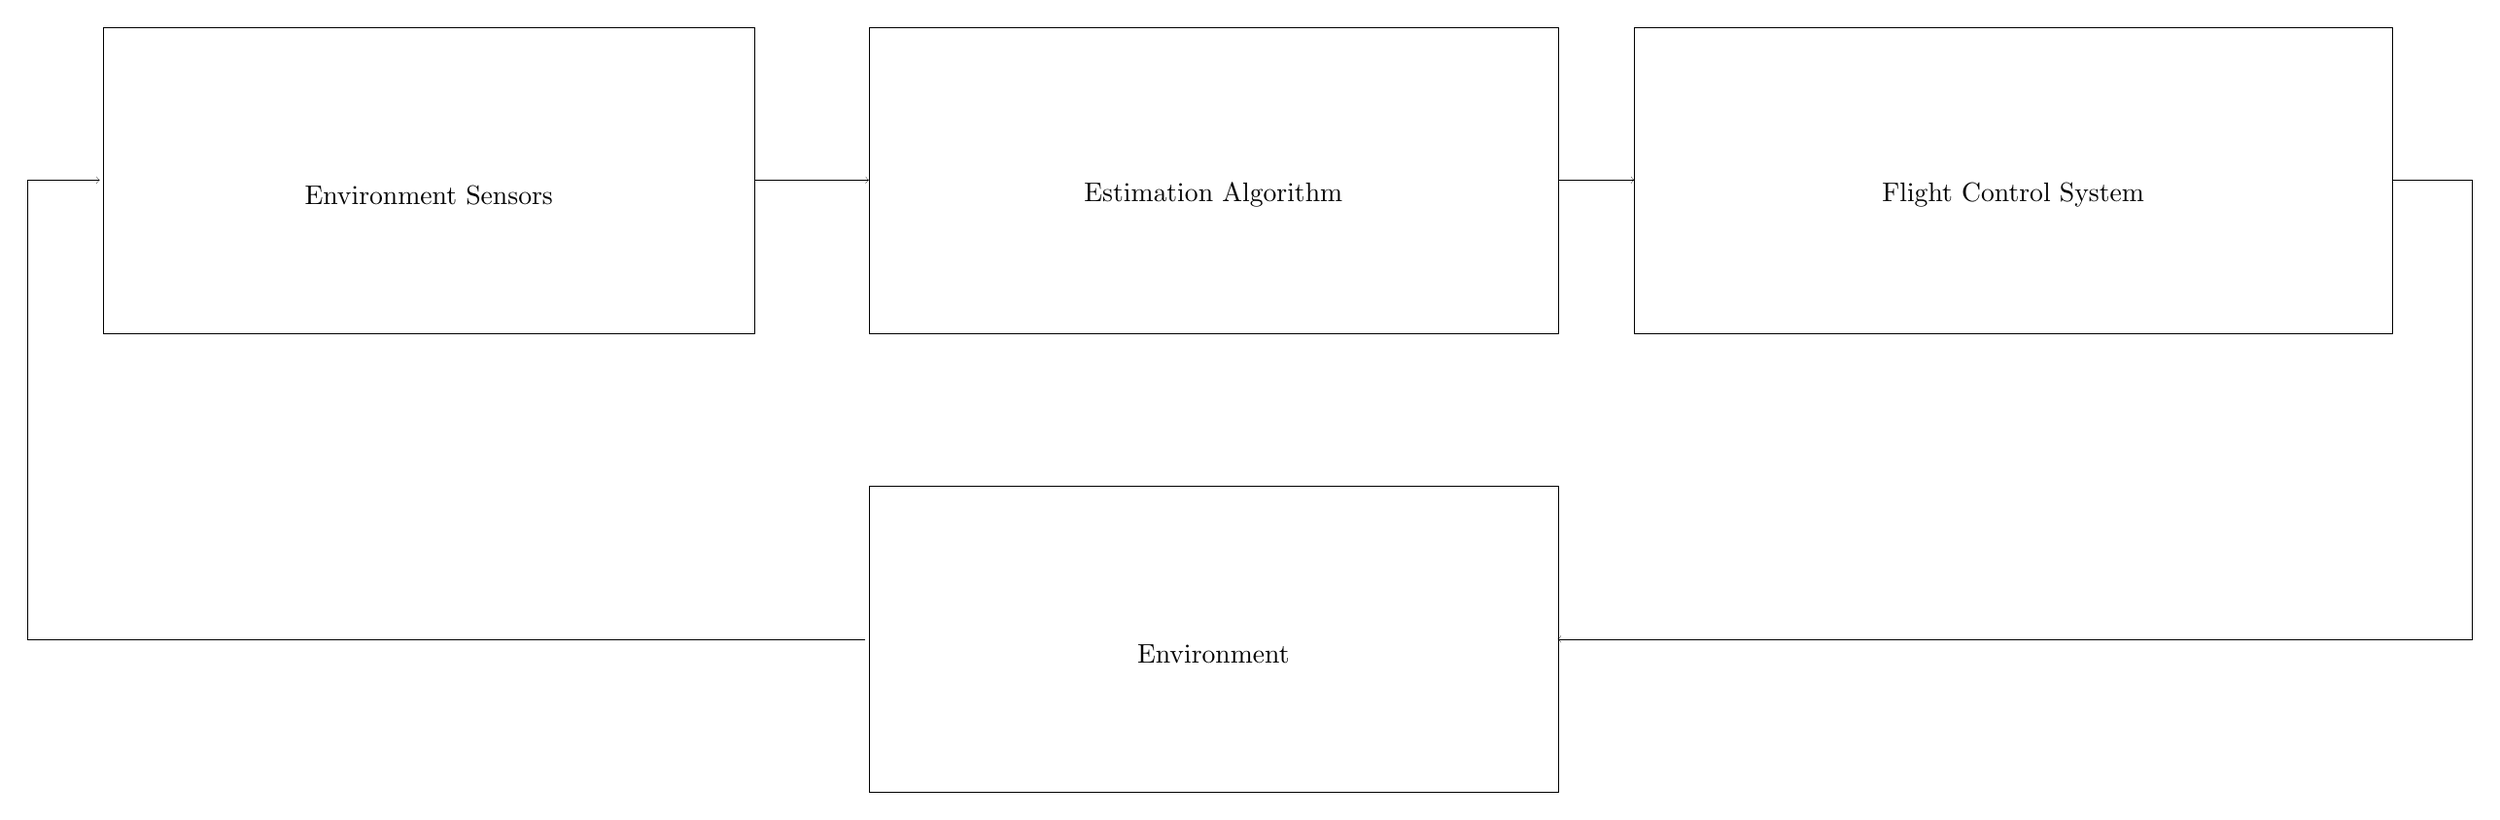
\begin{tikzpicture}
\pgftransformxscale{1.000000}
\pgftransformyscale{-1.000000}
\definecolor{dialinecolor}{rgb}{0.000000, 0.000000, 0.000000}
\pgfsetstrokecolor{dialinecolor}
\definecolor{dialinecolor}{rgb}{1.000000, 1.000000, 1.000000}
\pgfsetfillcolor{dialinecolor}
\definecolor{dialinecolor}{rgb}{1.000000, 1.000000, 1.000000}
\pgfsetfillcolor{dialinecolor}
\fill (18.000000\du,20.000000\du)--(18.000000\du,24.000000\du)--(27.000000\du,24.000000\du)--(27.000000\du,20.000000\du)--cycle;
\pgfsetlinewidth{0.100000\du}
\pgfsetdash{}{0pt}
\pgfsetdash{}{0pt}
\pgfsetmiterjoin
\definecolor{dialinecolor}{rgb}{0.000000, 0.000000, 0.000000}
\pgfsetstrokecolor{dialinecolor}
\draw (18.000000\du,20.000000\du)--(18.000000\du,24.000000\du)--(27.000000\du,24.000000\du)--(27.000000\du,20.000000\du)--cycle;
% setfont left to latex
\definecolor{dialinecolor}{rgb}{0.000000, 0.000000, 0.000000}
\pgfsetstrokecolor{dialinecolor}
\node at (22.500000\du,22.195000\du){Estimation Algorithm};
\definecolor{dialinecolor}{rgb}{1.000000, 1.000000, 1.000000}
\pgfsetfillcolor{dialinecolor}
\fill (28.000000\du,20.000000\du)--(28.000000\du,24.000000\du)--(37.900000\du,24.000000\du)--(37.900000\du,20.000000\du)--cycle;
\pgfsetlinewidth{0.100000\du}
\pgfsetdash{}{0pt}
\pgfsetdash{}{0pt}
\pgfsetmiterjoin
\definecolor{dialinecolor}{rgb}{0.000000, 0.000000, 0.000000}
\pgfsetstrokecolor{dialinecolor}
\draw (28.000000\du,20.000000\du)--(28.000000\du,24.000000\du)--(37.900000\du,24.000000\du)--(37.900000\du,20.000000\du)--cycle;
% setfont left to latex
\definecolor{dialinecolor}{rgb}{0.000000, 0.000000, 0.000000}
\pgfsetstrokecolor{dialinecolor}
\node at (32.950000\du,22.195000\du){Flight Control System};
\definecolor{dialinecolor}{rgb}{1.000000, 1.000000, 1.000000}
\pgfsetfillcolor{dialinecolor}
\fill (8.000000\du,20.000000\du)--(8.000000\du,24.000000\du)--(16.500000\du,24.000000\du)--(16.500000\du,20.000000\du)--cycle;
\pgfsetlinewidth{0.100000\du}
\pgfsetdash{}{0pt}
\pgfsetdash{}{0pt}
\pgfsetmiterjoin
\definecolor{dialinecolor}{rgb}{0.000000, 0.000000, 0.000000}
\pgfsetstrokecolor{dialinecolor}
\draw (8.000000\du,20.000000\du)--(8.000000\du,24.000000\du)--(16.500000\du,24.000000\du)--(16.500000\du,20.000000\du)--cycle;
% setfont left to latex
\definecolor{dialinecolor}{rgb}{0.000000, 0.000000, 0.000000}
\pgfsetstrokecolor{dialinecolor}
\node at (12.250000\du,22.195000\du){Environment Sensors};
\pgfsetlinewidth{0.100000\du}
\pgfsetdash{}{0pt}
\pgfsetdash{}{0pt}
\pgfsetbuttcap
{
\definecolor{dialinecolor}{rgb}{0.000000, 0.000000, 0.000000}
\pgfsetfillcolor{dialinecolor}
% was here!!!
\pgfsetarrowsend{to}
\definecolor{dialinecolor}{rgb}{0.000000, 0.000000, 0.000000}
\pgfsetstrokecolor{dialinecolor}
\draw (16.500000\du,22.000000\du)--(18.000000\du,22.000000\du);
}
\pgfsetlinewidth{0.100000\du}
\pgfsetdash{}{0pt}
\pgfsetdash{}{0pt}
\pgfsetbuttcap
{
\definecolor{dialinecolor}{rgb}{0.000000, 0.000000, 0.000000}
\pgfsetfillcolor{dialinecolor}
% was here!!!
\pgfsetarrowsend{to}
\definecolor{dialinecolor}{rgb}{0.000000, 0.000000, 0.000000}
\pgfsetstrokecolor{dialinecolor}
\draw (27.000000\du,22.000000\du)--(28.000000\du,22.000000\du);
}
\definecolor{dialinecolor}{rgb}{1.000000, 1.000000, 1.000000}
\pgfsetfillcolor{dialinecolor}
\fill (18.000000\du,26.000000\du)--(18.000000\du,30.000000\du)--(27.000000\du,30.000000\du)--(27.000000\du,26.000000\du)--cycle;
\pgfsetlinewidth{0.100000\du}
\pgfsetdash{}{0pt}
\pgfsetdash{}{0pt}
\pgfsetmiterjoin
\definecolor{dialinecolor}{rgb}{0.000000, 0.000000, 0.000000}
\pgfsetstrokecolor{dialinecolor}
\draw (18.000000\du,26.000000\du)--(18.000000\du,30.000000\du)--(27.000000\du,30.000000\du)--(27.000000\du,26.000000\du)--cycle;
% setfont left to latex
\definecolor{dialinecolor}{rgb}{0.000000, 0.000000, 0.000000}
\pgfsetstrokecolor{dialinecolor}
\node at (22.500000\du,28.195000\du){Environment};
\pgfsetlinewidth{0.100000\du}
\pgfsetdash{}{0pt}
\pgfsetdash{}{0pt}
\pgfsetmiterjoin
\pgfsetbuttcap
{
\definecolor{dialinecolor}{rgb}{0.000000, 0.000000, 0.000000}
\pgfsetfillcolor{dialinecolor}
% was here!!!
\pgfsetarrowsend{to}
{\pgfsetcornersarced{\pgfpoint{0.000000\du}{0.000000\du}}\definecolor{dialinecolor}{rgb}{0.000000, 0.000000, 0.000000}
\pgfsetstrokecolor{dialinecolor}
\draw (37.900000\du,22.000000\du)--(38.950000\du,22.000000\du)--(38.950000\du,28.000000\du)--(27.000000\du,28.000000\du);
}}
\pgfsetlinewidth{0.100000\du}
\pgfsetdash{}{0pt}
\pgfsetdash{}{0pt}
\pgfsetmiterjoin
\pgfsetbuttcap
{
\definecolor{dialinecolor}{rgb}{0.000000, 0.000000, 0.000000}
\pgfsetfillcolor{dialinecolor}
% was here!!!
\pgfsetarrowsend{to}
{\pgfsetcornersarced{\pgfpoint{0.000000\du}{0.000000\du}}\definecolor{dialinecolor}{rgb}{0.000000, 0.000000, 0.000000}
\pgfsetstrokecolor{dialinecolor}
\draw (17.950470\du,28.000000\du)--(7.000000\du,28.000000\du)--(7.000000\du,22.000000\du)--(7.950409\du,22.000000\du);
}}
\end{tikzpicture}

	\caption{Role of estimation algorithm\label{fig:estAlg1}}
\end{figure}

This section outlines the design process undertaken in selecting the estimation algorithm, and a brief overview of the final algorithm selected. 

\subsection{Pre-existing solutions for localising UAVs}
In the above discussion, it was mentioned that sensor data needs to be used to interpret both URSA's location and surroundings. The location aspect of this may be surprising, since there are many commercially available UAVs (including very cheap options) which are already able to fully automate position control. This includes, for example, following a flight plan specified by waypoints, circling a designated object, or holding a given position\footnote{See for example, the advertised capabilities of the 3DR SOLO or the DJI Phantom Series, both of which are cheap UAVs which provide these capabilities}. It may be expected that URSA can simply duplicate an existing solution for the localisation aspect of the algorithm, leaving obstacle detection and avoidance as a seperate and additional system.\\

However, this is not possible for the reasons which will be outlined below. Nevertheless, it is worth exploring the current approach taken by designers of commercial UAVs for the purposes of positional automation. This will further clarify the role of the estimation algorithm in the context of URSA.\\

The relevant data typically available to a UAV to allow localisation is some combination of the following:
\begin{itemize}
	\item GPS coordinates
	\item 3-axis Compass
	\item 3-axis Accelerometer
	\item 3-axis Gyroscope
	\item Barometer
\end{itemize}

This data is usually fused using a simple filter (such as an averaging filter) or a more advanced approach such as an EKF to remove noise and provide an estimate. In some systems, the attitude (or orientation) of the drone is calculated seperately to the position of the drone - however typically the best results are obtained by fusing all sensor data into a joint attitude/positional estimate. The output of this fusing can then be used as feedback to a PID controller to allow control of the drone. Often there are seperate PID controllers for both position and velocity to allow maximum flexibility in controlling the UAV. One possible implementation which may be found on a commercial drone is shown at Figure \ref{fig:estAlg2}. \\

This is usually a good approach for localisation since the data from the IMU, Compass, and Barometer are very sensitive to minor, rapid changes in attitude or position. By fusing this information with the slower but highly accurate GPS data, the system attains better positional resolution and is able to respond faster to environmental changes. For example, if a gust of wind suddenly pushes a UAV off course, it is unlikely that the GPS will update fast enough to allow the actuators to correct for this. Relying on GPS data alone in this case could cause instability by oscillating due to delays in the GPS signal. By obtaining a fused estimate, the data becomes appropriate to feed into a more sensitive PID controller which can respond rapidly to environmental changes.

\begin{figure}[H]
	% Graphic for TeX using PGF
% Title: /home/lach/uni/ursa/estimationAlg_Fig2
% Creator: Dia v0.97.3
% CreationDate: Sun Sep 17 11:12:20 2017
% For: lach
% \usepackage{tikz}
% The following commands are not supported in PSTricks at present
% We define them conditionally, so when they are implemented,
% this pgf file will use them.
\ifx\du\undefined
  \newlength{\du}
\fi
\setlength{\du}{15\unitlength}
\begin{tikzpicture}
\pgftransformxscale{1.000000}
\pgftransformyscale{-1.000000}
\definecolor{dialinecolor}{rgb}{0.000000, 0.000000, 0.000000}
\pgfsetstrokecolor{dialinecolor}
\definecolor{dialinecolor}{rgb}{1.000000, 1.000000, 1.000000}
\pgfsetfillcolor{dialinecolor}
\definecolor{dialinecolor}{rgb}{1.000000, 1.000000, 1.000000}
\pgfsetfillcolor{dialinecolor}
\fill (18.000000\du,20.000000\du)--(18.000000\du,24.000000\du)--(27.000000\du,24.000000\du)--(27.000000\du,20.000000\du)--cycle;
\pgfsetlinewidth{0.100000\du}
\pgfsetdash{}{0pt}
\pgfsetdash{}{0pt}
\pgfsetmiterjoin
\definecolor{dialinecolor}{rgb}{0.000000, 0.000000, 0.000000}
\pgfsetstrokecolor{dialinecolor}
\draw (18.000000\du,20.000000\du)--(18.000000\du,24.000000\du)--(27.000000\du,24.000000\du)--(27.000000\du,20.000000\du)--cycle;
% setfont left to latex
\definecolor{dialinecolor}{rgb}{0.000000, 0.000000, 0.000000}
\pgfsetstrokecolor{dialinecolor}
\node at (22.500000\du,22.195000\du){EKF};
\definecolor{dialinecolor}{rgb}{1.000000, 1.000000, 1.000000}
\pgfsetfillcolor{dialinecolor}
\fill (28.000000\du,20.000000\du)--(28.000000\du,24.000000\du)--(37.900000\du,24.000000\du)--(37.900000\du,20.000000\du)--cycle;
\pgfsetlinewidth{0.100000\du}
\pgfsetdash{}{0pt}
\pgfsetdash{}{0pt}
\pgfsetmiterjoin
\definecolor{dialinecolor}{rgb}{0.000000, 0.000000, 0.000000}
\pgfsetstrokecolor{dialinecolor}
\draw (28.000000\du,20.000000\du)--(28.000000\du,24.000000\du)--(37.900000\du,24.000000\du)--(37.900000\du,20.000000\du)--cycle;
% setfont left to latex
\definecolor{dialinecolor}{rgb}{0.000000, 0.000000, 0.000000}
\pgfsetstrokecolor{dialinecolor}
\node at (32.950000\du,22.195000\du){PID};
\definecolor{dialinecolor}{rgb}{1.000000, 1.000000, 1.000000}
\pgfsetfillcolor{dialinecolor}
\fill (8.000000\du,20.000000\du)--(8.000000\du,24.000000\du)--(16.500000\du,24.000000\du)--(16.500000\du,20.000000\du)--cycle;
\pgfsetlinewidth{0.100000\du}
\pgfsetdash{}{0pt}
\pgfsetdash{}{0pt}
\pgfsetmiterjoin
\definecolor{dialinecolor}{rgb}{0.000000, 0.000000, 0.000000}
\pgfsetstrokecolor{dialinecolor}
\draw (8.000000\du,20.000000\du)--(8.000000\du,24.000000\du)--(16.500000\du,24.000000\du)--(16.500000\du,20.000000\du)--cycle;
% setfont left to latex
\definecolor{dialinecolor}{rgb}{0.000000, 0.000000, 0.000000}
\pgfsetstrokecolor{dialinecolor}
\node at (12.250000\du,22.195000\du){Compass};
\pgfsetlinewidth{0.100000\du}
\pgfsetdash{}{0pt}
\pgfsetdash{}{0pt}
\pgfsetbuttcap
{
\definecolor{dialinecolor}{rgb}{0.000000, 0.000000, 0.000000}
\pgfsetfillcolor{dialinecolor}
% was here!!!
\pgfsetarrowsend{to}
\definecolor{dialinecolor}{rgb}{0.000000, 0.000000, 0.000000}
\pgfsetstrokecolor{dialinecolor}
\draw (16.500000\du,22.000000\du)--(18.000000\du,22.000000\du);
}
\pgfsetlinewidth{0.100000\du}
\pgfsetdash{}{0pt}
\pgfsetdash{}{0pt}
\pgfsetbuttcap
{
\definecolor{dialinecolor}{rgb}{0.000000, 0.000000, 0.000000}
\pgfsetfillcolor{dialinecolor}
% was here!!!
\pgfsetarrowsend{to}
\definecolor{dialinecolor}{rgb}{0.000000, 0.000000, 0.000000}
\pgfsetstrokecolor{dialinecolor}
\draw (27.000000\du,22.000000\du)--(28.000000\du,22.000000\du);
}
\definecolor{dialinecolor}{rgb}{1.000000, 1.000000, 1.000000}
\pgfsetfillcolor{dialinecolor}
\fill (28.000000\du,26.000000\du)--(28.000000\du,30.000000\du)--(38.000000\du,30.000000\du)--(38.000000\du,26.000000\du)--cycle;
\pgfsetlinewidth{0.100000\du}
\pgfsetdash{}{0pt}
\pgfsetdash{}{0pt}
\pgfsetmiterjoin
\definecolor{dialinecolor}{rgb}{0.000000, 0.000000, 0.000000}
\pgfsetstrokecolor{dialinecolor}
\draw (28.000000\du,26.000000\du)--(28.000000\du,30.000000\du)--(38.000000\du,30.000000\du)--(38.000000\du,26.000000\du)--cycle;
% setfont left to latex
\definecolor{dialinecolor}{rgb}{0.000000, 0.000000, 0.000000}
\pgfsetstrokecolor{dialinecolor}
\node at (33.000000\du,28.195000\du){Actuators};
\definecolor{dialinecolor}{rgb}{1.000000, 1.000000, 1.000000}
\pgfsetfillcolor{dialinecolor}
\fill (8.000000\du,15.000000\du)--(8.000000\du,19.000000\du)--(16.500000\du,19.000000\du)--(16.500000\du,15.000000\du)--cycle;
\pgfsetlinewidth{0.100000\du}
\pgfsetdash{}{0pt}
\pgfsetdash{}{0pt}
\pgfsetmiterjoin
\definecolor{dialinecolor}{rgb}{0.000000, 0.000000, 0.000000}
\pgfsetstrokecolor{dialinecolor}
\draw (8.000000\du,15.000000\du)--(8.000000\du,19.000000\du)--(16.500000\du,19.000000\du)--(16.500000\du,15.000000\du)--cycle;
% setfont left to latex
\definecolor{dialinecolor}{rgb}{0.000000, 0.000000, 0.000000}
\pgfsetstrokecolor{dialinecolor}
\node at (12.250000\du,17.195000\du){GPS Data};
\definecolor{dialinecolor}{rgb}{1.000000, 1.000000, 1.000000}
\pgfsetfillcolor{dialinecolor}
\fill (8.000000\du,25.000000\du)--(8.000000\du,29.000000\du)--(16.500000\du,29.000000\du)--(16.500000\du,25.000000\du)--cycle;
\pgfsetlinewidth{0.100000\du}
\pgfsetdash{}{0pt}
\pgfsetdash{}{0pt}
\pgfsetmiterjoin
\definecolor{dialinecolor}{rgb}{0.000000, 0.000000, 0.000000}
\pgfsetstrokecolor{dialinecolor}
\draw (8.000000\du,25.000000\du)--(8.000000\du,29.000000\du)--(16.500000\du,29.000000\du)--(16.500000\du,25.000000\du)--cycle;
% setfont left to latex
\definecolor{dialinecolor}{rgb}{0.000000, 0.000000, 0.000000}
\pgfsetstrokecolor{dialinecolor}
\node at (12.250000\du,27.195000\du){IMU/Baro};
\pgfsetlinewidth{0.100000\du}
\pgfsetdash{}{0pt}
\pgfsetdash{}{0pt}
\pgfsetmiterjoin
\pgfsetbuttcap
{
\definecolor{dialinecolor}{rgb}{0.000000, 0.000000, 0.000000}
\pgfsetfillcolor{dialinecolor}
% was here!!!
\pgfsetarrowsend{to}
{\pgfsetcornersarced{\pgfpoint{0.000000\du}{0.000000\du}}\definecolor{dialinecolor}{rgb}{0.000000, 0.000000, 0.000000}
\pgfsetstrokecolor{dialinecolor}
\draw (16.550262\du,17.000000\du)--(22.500000\du,17.000000\du)--(22.500000\du,20.000000\du);
}}
\pgfsetlinewidth{0.100000\du}
\pgfsetdash{}{0pt}
\pgfsetdash{}{0pt}
\pgfsetmiterjoin
\pgfsetbuttcap
{
\definecolor{dialinecolor}{rgb}{0.000000, 0.000000, 0.000000}
\pgfsetfillcolor{dialinecolor}
% was here!!!
\pgfsetarrowsend{to}
{\pgfsetcornersarced{\pgfpoint{0.000000\du}{0.000000\du}}\definecolor{dialinecolor}{rgb}{0.000000, 0.000000, 0.000000}
\pgfsetstrokecolor{dialinecolor}
\draw (16.550262\du,27.000000\du)--(22.500000\du,27.000000\du)--(22.500000\du,24.000000\du);
}}
\pgfsetlinewidth{0.100000\du}
\pgfsetdash{}{0pt}
\pgfsetdash{}{0pt}
\pgfsetbuttcap
{
\definecolor{dialinecolor}{rgb}{0.000000, 0.000000, 0.000000}
\pgfsetfillcolor{dialinecolor}
% was here!!!
\pgfsetarrowsend{to}
\definecolor{dialinecolor}{rgb}{0.000000, 0.000000, 0.000000}
\pgfsetstrokecolor{dialinecolor}
\draw (32.950000\du,24.000000\du)--(33.000000\du,26.000000\du);
}
\end{tikzpicture}

	\caption{Simplified diagram of existing positional estimation\label{fig:estAlg2}}
\end{figure}

However, this approach cannot be applied to URSA. This is because in an indoor environment, GPS data is not generally available, and when the GPS data is available it is extremely inaccurate. GPS relies on unobstructed signal paths to a satellite. Indoors, GPS signals are usually obtained by reflection off surrounding objects. This changes the signal path lengths in unpredictable ways, and the data becomes unusable. Obtaining a reliable GPS signal indoors is an active area of research. The current state of this research suggests using indoor repeaters designed specifically for the space \cite{ozsoy}. This is obviously not practicable in an emergency situation, as these repeaters would likely not already be installed, or may be subject to failure. \\

It may seem counterintuitive that a loss of one sensor (i.e. GPS) in Figure \ref{fig:estAlg2} would destroy the accuracy of the system. One of the advantages of fusing multiple sensors is in adding system redundancy. If one of the sensors fails, it is expected that the other sensors will still provide a good estimate of the attitude and position of the UAV. The reason why the system will fail without GPS can be seen by inspecting the remaining sensors. Critically, there are no remaining sources of direct latitude/longditude information, so the system will eventually accumulate error over time. \\

The IMU provides us with a measurement of the second derivative of these values, however to obtain the position we then have to integrate these measurements twice. This procedure is known as `dead-reckoning', and has been used in navigation for several centuries. Dead-reckoning has the well-known drawback that errors are cumulative, so they continue to increase with each subsequent measurement. It is also clear that some error is unavoidable - even if our sensors were perfectly accurate, they are digital sensors which only provide a limited resolution in both time and amplitude. In reality, they are also not perfectly accurate, exhibiting biases even after calibration. If we consider just the case of a small bias, the cumulative nature of the estimation error can be shown by the following example.\\ 

Assume the bias does not change with time, and is a random variable $B$ with $E[B]=0$. Therefore, the reading in one dimension $x$ at time step $t$ is $Y=\ddot{x}+B$, where $\ddot{x}$ is the acceleration reading parallel to $x$. The optimal estimate of $\ddot{x}$ is $Y$. Assuming zero starting position and velocity, and motion in a straight line, we can then write the optimal estimator of $\hat{x}_{pos}$ as:

\begin{align*}
	\hat{x}_{pos}(0)&=\frac{1}{2}y(0)\Delta t^2\\
	&=\frac{1}{2}(\ddot{x}(0)+B)\Delta t^2\\
\end{align*}

Which clearly has an error term of $B\Delta t^2$. The estimate gets worse as we continue to integrate:

\begin{align*}
\hat{x}_{pos}(1)&=\frac{1}{2}y(1)\Delta t^2+y(0)\Delta t^2+\frac{1}{2}y(0)\Delta t^2\\
&=\frac{1}{2}(\ddot{x}(1)+B)\Delta t^2+\frac{3}{2}(\ddot{x}(0)+B)\Delta t^2\\   	
\end{align*}

Which has an error term of $2B\Delta t^2$. Therefore we see that even a minor bias will grow linearly with the square of the sampling period. This is known as a `cumulative' error. This effect was confirmed experimentally by providing just the IMU data to the URSA flight controller. We observed a constant `drift' when the controller attempted to maintain a given position.\\

At time $t$ the error is then:

\begin{align*} 
	E_x=&\frac{t}{\Delta t}B\Delta t^2\\
	=&tB\Delta t
\end{align*}

We can reduce the impact of this bias by reducing our sampling period, $\Delta t$ or the offset bias, B. B could be reduced by, for example, purchasing a more expensive and finely calibrated IMU. However, even with extremely fast sampling or low error, there will be some time $t$ for which the error is unacceptable.\\

The solution to this problem is to have a reliable positional estimate which does not exhibit cumulative errors. Our system therefore needs a source of positional data which does not exhibit cumulative errors, which can be used to correct for cumulative errors in other sensors. \\

We therefore need a solution to replace the GPS data source used in commercial UAVs, which will function indoors. This is one of the roles which will be filled by the estimation algorithm. The other role will be to map obstacles for the purpose of obstacle avoidance. A modified version of Figure \ref{fig:estAlg2} reflecting the role of this estimation algorithm is shown at Figure \ref{fig:estAlg3}.\\

In Figure \ref{fig:estAlg3}, the following system blocks merit some additional explanation for the sake of clarity:
\begin{enumerate}
	\item \textbf{Non cumulative error (NCE) estimation algorithm:} A SLAM algorithm which can take sensor readings and output an estimate of the current position which does not accumulate error with time, as well as an estimate of static obstacles.
	\item \textbf{Additional sensors:} Whatever additional sensors may be required for the SLAM algorithm. These will depend on the algorithm chosen and so are intentionally left general. In the case of URSA, we chose a SLAM algorithm which requires laser scan data. This is discussed further below.
	\item \textbf{EKF:} An estimation filter which fuses together different measurements into a state estimation. We are treating the position output of the NCE estimator as a single measurement from an observation model. The IMU data (linear and angular acceleration) is another measurement under the observation model. The process and advantages of fusing together these measurements is discussed earlier in this Chapter. The implementation of this filter is discussed in the next chapter.
	\item \textbf{PID:} A controller which accepts a state estimation from the EKF and a setpoint from the autonomous navigation algorithm, and provides signals to the actuators (being the four rotors of the UAV) which attempt to fly the UAV to the setpoint position and attitude.
\end{enumerate}

In some indoor UAV implementations, devices which use optical flow have been developed to provide positional estimates in place of GPS sensors. The premise is that visible spectrum cameras are pointed directly at the floor. Subsequent frames are searched for offsets, which can be converted to velocity measurements. These velocity measurements typically have very little noise and no bias, so can be integrated without such a large error as described in the inertial case. An example of this type of device is the PX4FLOW sensor board \footnote{\url{https://pixhawk.org/dev/px4flow}}. \\

This is typically a very robust approach to localisation. However, it has not been considered for URSA for two reasons: as with all visible light optical techniques, it is reliant on good lighting of the scene. This cannot be guaranteed in an emergency situation. A light source could be included on URSA, however this can cause flow calculations to be distorted by direct lighting and shadow casting on some surfaces.\\

The second reason an optical flow sensor not appropriate to URSA is that it only solves the problem of localisation. The requirement remains to map URSA's surroundings in order to navigate. As will be seen, both localization and mapping can (and should) be solved simultaneously with one algorithm, rendering the flow sensor redundant. It may be the case that this redundancy is desirable. In a commercial or high-reliability situation which is required to be robust to one estimation method failing, an optical flow sensor may also be included. In our case, we are simply developing a prototype, and so haven't integrated a flow sensor.

    \begin{figure}[H]
    	\centering
    	% Graphic for TeX using PGF
% Title: /home/lach/uni/ursa/final_report/diagrams/estimationAlg_Fig3.dia
% Creator: Dia v0.97.3
% CreationDate: Tue Oct 24 18:45:33 2017
% For: lach
% \usepackage{tikz}
% The following commands are not supported in PSTricks at present
% We define them conditionally, so when they are implemented,
% this pgf file will use them.
\ifx\du\undefined
  \newlength{\du}
\fi
\setlength{\du}{15\unitlength}
\begin{tikzpicture}
\pgftransformxscale{1.000000}
\pgftransformyscale{-1.000000}
\definecolor{dialinecolor}{rgb}{0.000000, 0.000000, 0.000000}
\pgfsetstrokecolor{dialinecolor}
\definecolor{dialinecolor}{rgb}{1.000000, 1.000000, 1.000000}
\pgfsetfillcolor{dialinecolor}
\definecolor{dialinecolor}{rgb}{1.000000, 1.000000, 1.000000}
\pgfsetfillcolor{dialinecolor}
\fill (18.000000\du,20.000000\du)--(18.000000\du,24.000000\du)--(27.000000\du,24.000000\du)--(27.000000\du,20.000000\du)--cycle;
\pgfsetlinewidth{0.100000\du}
\pgfsetdash{}{0pt}
\pgfsetdash{}{0pt}
\pgfsetmiterjoin
\definecolor{dialinecolor}{rgb}{0.000000, 0.000000, 0.000000}
\pgfsetstrokecolor{dialinecolor}
\draw (18.000000\du,20.000000\du)--(18.000000\du,24.000000\du)--(27.000000\du,24.000000\du)--(27.000000\du,20.000000\du)--cycle;
% setfont left to latex
\definecolor{dialinecolor}{rgb}{0.000000, 0.000000, 0.000000}
\pgfsetstrokecolor{dialinecolor}
\node at (22.500000\du,22.195000\du){EKF};
\definecolor{dialinecolor}{rgb}{1.000000, 1.000000, 1.000000}
\pgfsetfillcolor{dialinecolor}
\fill (28.000000\du,20.000000\du)--(28.000000\du,24.000000\du)--(37.900000\du,24.000000\du)--(37.900000\du,20.000000\du)--cycle;
\pgfsetlinewidth{0.100000\du}
\pgfsetdash{}{0pt}
\pgfsetdash{}{0pt}
\pgfsetmiterjoin
\definecolor{dialinecolor}{rgb}{0.000000, 0.000000, 0.000000}
\pgfsetstrokecolor{dialinecolor}
\draw (28.000000\du,20.000000\du)--(28.000000\du,24.000000\du)--(37.900000\du,24.000000\du)--(37.900000\du,20.000000\du)--cycle;
% setfont left to latex
\definecolor{dialinecolor}{rgb}{0.000000, 0.000000, 0.000000}
\pgfsetstrokecolor{dialinecolor}
\node at (32.950000\du,22.195000\du){PID};
\pgfsetlinewidth{0.100000\du}
\pgfsetdash{}{0pt}
\pgfsetdash{}{0pt}
\pgfsetbuttcap
{
\definecolor{dialinecolor}{rgb}{0.000000, 0.000000, 0.000000}
\pgfsetfillcolor{dialinecolor}
% was here!!!
\pgfsetarrowsend{to}
\definecolor{dialinecolor}{rgb}{0.000000, 0.000000, 0.000000}
\pgfsetstrokecolor{dialinecolor}
\draw (27.000000\du,22.000000\du)--(28.000000\du,22.000000\du);
}
\definecolor{dialinecolor}{rgb}{1.000000, 1.000000, 1.000000}
\pgfsetfillcolor{dialinecolor}
\fill (28.000000\du,26.000000\du)--(28.000000\du,30.000000\du)--(38.000000\du,30.000000\du)--(38.000000\du,26.000000\du)--cycle;
\pgfsetlinewidth{0.100000\du}
\pgfsetdash{}{0pt}
\pgfsetdash{}{0pt}
\pgfsetmiterjoin
\definecolor{dialinecolor}{rgb}{0.000000, 0.000000, 0.000000}
\pgfsetstrokecolor{dialinecolor}
\draw (28.000000\du,26.000000\du)--(28.000000\du,30.000000\du)--(38.000000\du,30.000000\du)--(38.000000\du,26.000000\du)--cycle;
% setfont left to latex
\definecolor{dialinecolor}{rgb}{0.000000, 0.000000, 0.000000}
\pgfsetstrokecolor{dialinecolor}
\node at (33.000000\du,28.195000\du){Actuators};
\definecolor{dialinecolor}{rgb}{1.000000, 1.000000, 1.000000}
\pgfsetfillcolor{dialinecolor}
\fill (8.000000\du,15.000000\du)--(8.000000\du,19.000000\du)--(16.500000\du,19.000000\du)--(16.500000\du,15.000000\du)--cycle;
\pgfsetlinewidth{0.100000\du}
\pgfsetdash{}{0pt}
\pgfsetdash{}{0pt}
\pgfsetmiterjoin
\definecolor{dialinecolor}{rgb}{0.000000, 0.000000, 0.000000}
\pgfsetstrokecolor{dialinecolor}
\draw (8.000000\du,15.000000\du)--(8.000000\du,19.000000\du)--(16.500000\du,19.000000\du)--(16.500000\du,15.000000\du)--cycle;
% setfont left to latex
\definecolor{dialinecolor}{rgb}{0.000000, 0.000000, 0.000000}
\pgfsetstrokecolor{dialinecolor}
\node at (12.250000\du,16.795000\du){NCE};
% setfont left to latex
\definecolor{dialinecolor}{rgb}{0.000000, 0.000000, 0.000000}
\pgfsetstrokecolor{dialinecolor}
\node at (12.250000\du,17.595000\du){Estimation Algorithm};
\definecolor{dialinecolor}{rgb}{1.000000, 1.000000, 1.000000}
\pgfsetfillcolor{dialinecolor}
\fill (8.000000\du,25.000000\du)--(8.000000\du,29.000000\du)--(16.500000\du,29.000000\du)--(16.500000\du,25.000000\du)--cycle;
\pgfsetlinewidth{0.100000\du}
\pgfsetdash{}{0pt}
\pgfsetdash{}{0pt}
\pgfsetmiterjoin
\definecolor{dialinecolor}{rgb}{0.000000, 0.000000, 0.000000}
\pgfsetstrokecolor{dialinecolor}
\draw (8.000000\du,25.000000\du)--(8.000000\du,29.000000\du)--(16.500000\du,29.000000\du)--(16.500000\du,25.000000\du)--cycle;
% setfont left to latex
\definecolor{dialinecolor}{rgb}{0.000000, 0.000000, 0.000000}
\pgfsetstrokecolor{dialinecolor}
\node at (12.250000\du,27.195000\du){IMU};
\pgfsetlinewidth{0.100000\du}
\pgfsetdash{}{0pt}
\pgfsetdash{}{0pt}
\pgfsetmiterjoin
\pgfsetbuttcap
{
\definecolor{dialinecolor}{rgb}{0.000000, 0.000000, 0.000000}
\pgfsetfillcolor{dialinecolor}
% was here!!!
\pgfsetarrowsend{to}
{\pgfsetcornersarced{\pgfpoint{0.000000\du}{0.000000\du}}\definecolor{dialinecolor}{rgb}{0.000000, 0.000000, 0.000000}
\pgfsetstrokecolor{dialinecolor}
\draw (16.500000\du,18.000000\du)--(22.500000\du,18.000000\du)--(22.500000\du,20.000000\du);
}}
\pgfsetlinewidth{0.100000\du}
\pgfsetdash{}{0pt}
\pgfsetdash{}{0pt}
\pgfsetmiterjoin
\pgfsetbuttcap
{
\definecolor{dialinecolor}{rgb}{0.000000, 0.000000, 0.000000}
\pgfsetfillcolor{dialinecolor}
% was here!!!
\pgfsetarrowsend{to}
{\pgfsetcornersarced{\pgfpoint{0.000000\du}{0.000000\du}}\definecolor{dialinecolor}{rgb}{0.000000, 0.000000, 0.000000}
\pgfsetstrokecolor{dialinecolor}
\draw (16.550262\du,27.000000\du)--(22.500000\du,27.000000\du)--(22.500000\du,24.000000\du);
}}
\pgfsetlinewidth{0.100000\du}
\pgfsetdash{}{0pt}
\pgfsetdash{}{0pt}
\pgfsetbuttcap
{
\definecolor{dialinecolor}{rgb}{0.000000, 0.000000, 0.000000}
\pgfsetfillcolor{dialinecolor}
% was here!!!
\pgfsetarrowsend{to}
\definecolor{dialinecolor}{rgb}{0.000000, 0.000000, 0.000000}
\pgfsetstrokecolor{dialinecolor}
\draw (32.950000\du,24.000000\du)--(33.000000\du,26.000000\du);
}
\definecolor{dialinecolor}{rgb}{1.000000, 1.000000, 1.000000}
\pgfsetfillcolor{dialinecolor}
\fill (8.000000\du,10.000000\du)--(8.000000\du,14.000000\du)--(16.500000\du,14.000000\du)--(16.500000\du,10.000000\du)--cycle;
\pgfsetlinewidth{0.100000\du}
\pgfsetdash{}{0pt}
\pgfsetdash{}{0pt}
\pgfsetmiterjoin
\definecolor{dialinecolor}{rgb}{0.000000, 0.000000, 0.000000}
\pgfsetstrokecolor{dialinecolor}
\draw (8.000000\du,10.000000\du)--(8.000000\du,14.000000\du)--(16.500000\du,14.000000\du)--(16.500000\du,10.000000\du)--cycle;
% setfont left to latex
\definecolor{dialinecolor}{rgb}{0.000000, 0.000000, 0.000000}
\pgfsetstrokecolor{dialinecolor}
\node at (12.250000\du,12.195000\du){Additional Sensors};
\pgfsetlinewidth{0.100000\du}
\pgfsetdash{}{0pt}
\pgfsetdash{}{0pt}
\pgfsetbuttcap
{
\definecolor{dialinecolor}{rgb}{0.000000, 0.000000, 0.000000}
\pgfsetfillcolor{dialinecolor}
% was here!!!
\pgfsetarrowsend{to}
\definecolor{dialinecolor}{rgb}{0.000000, 0.000000, 0.000000}
\pgfsetstrokecolor{dialinecolor}
\draw (12.250000\du,14.041016\du)--(12.250000\du,14.958984\du);
}
\definecolor{dialinecolor}{rgb}{1.000000, 1.000000, 1.000000}
\pgfsetfillcolor{dialinecolor}
\fill (18.000000\du,10.000000\du)--(18.000000\du,14.000000\du)--(27.000000\du,14.000000\du)--(27.000000\du,10.000000\du)--cycle;
\pgfsetlinewidth{0.100000\du}
\pgfsetdash{}{0pt}
\pgfsetdash{}{0pt}
\pgfsetmiterjoin
\definecolor{dialinecolor}{rgb}{0.000000, 0.000000, 0.000000}
\pgfsetstrokecolor{dialinecolor}
\draw (18.000000\du,10.000000\du)--(18.000000\du,14.000000\du)--(27.000000\du,14.000000\du)--(27.000000\du,10.000000\du)--cycle;
% setfont left to latex
\definecolor{dialinecolor}{rgb}{0.000000, 0.000000, 0.000000}
\pgfsetstrokecolor{dialinecolor}
\node at (22.500000\du,12.195000\du){Navigation};
\pgfsetlinewidth{0.100000\du}
\pgfsetdash{}{0pt}
\pgfsetdash{}{0pt}
\pgfsetmiterjoin
\pgfsetbuttcap
{
\definecolor{dialinecolor}{rgb}{0.000000, 0.000000, 0.000000}
\pgfsetfillcolor{dialinecolor}
% was here!!!
\pgfsetarrowsend{to}
{\pgfsetcornersarced{\pgfpoint{0.000000\du}{0.000000\du}}\definecolor{dialinecolor}{rgb}{0.000000, 0.000000, 0.000000}
\pgfsetstrokecolor{dialinecolor}
\draw (16.500000\du,16.000000\du)--(22.500000\du,16.000000\du)--(22.500000\du,14.000000\du);
}}
\pgfsetlinewidth{0.100000\du}
\pgfsetdash{}{0pt}
\pgfsetdash{}{0pt}
\pgfsetmiterjoin
\pgfsetbuttcap
{
\definecolor{dialinecolor}{rgb}{0.000000, 0.000000, 0.000000}
\pgfsetfillcolor{dialinecolor}
% was here!!!
\pgfsetarrowsend{to}
{\pgfsetcornersarced{\pgfpoint{0.000000\du}{0.000000\du}}\definecolor{dialinecolor}{rgb}{0.000000, 0.000000, 0.000000}
\pgfsetstrokecolor{dialinecolor}
\draw (27.000000\du,12.000000\du)--(32.950000\du,12.000000\du)--(32.950000\du,20.000000\du);
}}
% setfont left to latex
\definecolor{dialinecolor}{rgb}{0.000000, 0.000000, 0.000000}
\pgfsetstrokecolor{dialinecolor}
\node[anchor=west] at (23.000000\du,18.500000\du){Position};
% setfont left to latex
\definecolor{dialinecolor}{rgb}{0.000000, 0.000000, 0.000000}
\pgfsetstrokecolor{dialinecolor}
\node[anchor=west] at (23.000000\du,15.500000\du){Obstacles};
\pgfsetlinewidth{0.100000\du}
\pgfsetdash{}{0pt}
\pgfsetdash{}{0pt}
\pgfsetbuttcap
{
\definecolor{dialinecolor}{rgb}{0.000000, 0.000000, 0.000000}
\pgfsetfillcolor{dialinecolor}
% was here!!!
\pgfsetarrowsend{to}
\definecolor{dialinecolor}{rgb}{0.000000, 0.000000, 0.000000}
\pgfsetstrokecolor{dialinecolor}
\draw (12.250000\du,25.000000\du)--(12.250000\du,19.000000\du);
}
\end{tikzpicture}

    	\caption{Non-cumulative error (NCE) estimator replacing GPS source for indoor flight\label{fig:estAlg3}}
    \end{figure}

\subsection{Requirements for algorithm}
Having identified the role the algorithm will play in our system, we can now formally document the major requirements of this algorithm. This list of requirements will be used in selecting and designing the algorithm. The major requirements of the estimation algorithm are as follows:

\begin{itemize}
	\item Real-time operation at approximately \SI{10}{\hertz}.
	\item Output both an estimation of URSA's location as well as a map of obstacles.
	\item Accuracy of at least $\pm \SI{0.5}{\meter}$.
	\item Capable of mapping obstacles in the immediate vicinity, and ideally creating a persistent map of these obstacles so the navigation system can `remember' the areas which have been explored.
	\item Capable of creating output from direct observations of a range of environments (i.e. visual, SONAR, LiDAR) rather than requiring transmitters to be set up.
	\item Compatible with sensors which can meet budget requirements.
\end{itemize}

These requirements are met generally by the family of algorithms known as SLAM, which were considered at a theoretical level in the literature review chapter.

\subsection{Final selection of algorithm}
We were able to compare a number of open source SLAM algorithms in order to determine the best estimation algorithm for our purposes. This process was greatly assisted by the website \url{https://openslam.org/}, which provides a platform for SLAM researchers to publish their algorithms. \\

This project is not intended to include an implementation or comprehensive evaluation of SLAM algorithms. However, we did download, configure and build the code for several open source SLAM algorithms on a desktop environment or in simulation. Performance was evaluated qualitatively based on limited datasets which were not controlled between each algorithm evaluated. The purpose was not to exhaustively evaluate the performance of each algorithm, but rather to find a solution which could be quickly configured and treated as a `black box' to allow us to achieve the system level objectives.\\


Some of the algorithms built by us and our qualitative conclusions are outlined in Table \ref{tab:slamAlg}.

\begin{table}[H]
	\centering
 	\begin{tabular}{|c|c|c|c|c|}
 		\hline
 		\bf{Algorithm Name}	&	\bf{Sensor Support}	&	\bf{Method}	&	\bf{Loop Closure?}\\
 		\hline
 		TinySLAM		&	Wheel odometry and laser scanner	&	Dense particle filter &	No\\	
 		\hline
 		ORB SLAM 	&		RGB camera & Sparse particle filter & Yes \\
 		\hline
 		RGBD SLAM & Depth Camera & Sparse EKF & Yes\\
 		\hline
 		Hector SLAM & Laser Scanner and IMU & Graph based & Yes\\
 		\hline
 		Cartographer & Laser Scanner and IMU & Graph based & Yes\\
 		\hline
 	\end{tabular}
 	\caption{Details of different SLAM algorithms considered and prototyped\label{tab:slamAlg}}
\end{table}

Some further information regarding our evaluation of these algorithms is provided below:
\begin{itemize}
	\item \bf{ORB SLAM} \normalfont- Tested with low resolution webcam. Quality of localisation found to be highly dependant on lighting conditions. Quality of mapping found to be poor under all conditions.
 	\item \bf{RGBD SLAM} \normalfont- Tested using a Microsoft Kinect. Found to provide very good localisation and 3D mapping - however the Kinect sensor is not suitable to be mounted on an average sized drone. Additionally, the memory requirements for large scale mapping were prohibitive.
 	\item \bf{Cartographer} \normalfont- Tested with pre-recorded laser scan data made available by the Cartographer authors\cite{cartdata}. Mapping and localisation found to be very good in 2D. Hardware requirements indicate that real-time performance would require a companion desktop machine.
\end{itemize}

Based on our assessment, we decided to use a 2D laser scanner and Cartographer to fulfill the requirements of our estimation algorithm. This required obtaining approval for the acquisition of a LiDAR scanner, which has a significant cost attached, however it is likely to be the only option which would allow the system to function correctly, and therefore has a clear business case. Further sensor details are discussed later in this report.\\

The two major drawbacks of selecting Cartographer are:

\begin{itemize}
 	\item The requirement to use a dedicated base-station for undertaking SLAM processing. This is likely mitigated by the fact that in a real-world scenario, a base station for deployment and control is likely desirable anyway.
 	\item An initial limitation to only 2D mapping. This means that the initial prototype of URSA will only be capable of navigation in a 2D plane at a set altitude. This has the effect of limiting the scope of navigation algorithms to 2D, which simplifies that aspect of the project. Ideally, URSA should be capable of flying both over/under and around obstacles. However, given the R\&D focus of this project, it is desirable to limit the scope of initial prototypes where possible, allowing expansion on this scope in future once the basic concepts have been proved.
\end{itemize}

The practical impact of the 2D limitation above is that we will also require an additional sensor for UAV height. Barometric pressure is unlikely to provide sufficient resolution, and in any case fluctuates considerably in an indoor environment. The selection of this sensor is discussed in the following section. \\

\section{Selection of sensor hardware}
In addition to the UAV itself, which is discussed previously, URSA will also require some additional sensor hardware in order for our NCE algorithm to function. It may seem that our choice of additional sensors beyond those already provided with the Erle-Copter was dictated by our choice of SLAM algorithm. In practice, there was interdependance between these decisions, so an analysis of sensor features was undertaken in parallel with SLAM algorithm selection. \\

Our relative value placed on sensor specifications are summarised in Table \ref{tab:sensors}.

\begin{table}[H]
\centering
\begin{tabular}{lp{6cm}p{3cm}}
\toprule
  Feature                                   & Description & Importance\\ 
\midrule
Light weight                                   & Greater payload, longer flight time & High \\
Low power consumption &	Greater battery life, flight duration and area covered. Generally good practice.	&High\\
Compact/low volume	&Easier to mount onto UAV, sensors less likely to interfere with propellers and other sensors.	&High\\
Reputable source	&Ensures quality of purchased products	&High\\
Open source driver software	&Saves time, potential for project scope to be expanded to achieve more UAV features with extra time.& Medium\\
Low cost	&Less sunk costs in the event of catastrophic failure, affordable replacement.	&Medium\\
Low CPU/memory requirement	&Frees up computational power for other functions.	&Medium\\
Fast shipping time &Reduced wait times, potential for project scope to be expanded to achieve more UAV features with extra time.	&Low\\
Robust	&Limits potential damage to the sensor	&Low \\
\bottomrule
\end{tabular}
\caption{Considerations for sensors\label{tab:sensors}}
\end{table}


With the above factors in mind, a range of active remote sensors are explored, with their suitability for our project assessed. Three families of sensors were found to be most suitable:

\begin{itemize}
\item Passive Visual: Passive visual sensors rely on the use of cameras and closely resembles human binocular vision; inferring 3D depth from the image output of two (or more) cameras. As such, passive visual sensors are dependent on external lighting and require an internal lighting mechanism in dark environments. They provide higher resolution at the expense of greater CPU memory requirements. 
\item LIDAR: Lidar (Light Detection And Ranging) is a sensing method that uses emitted laser pulses, processing correlation algorithms from the timing and phase-shift of their subsequent reflection off surfaces to determine distances/depth. In our application, LIDAR can be used to create 3D or 2D point clouds, so that the drone is able to calculate position while also identifying the presence of potential obstacles. Furthermore, these point clouds can be transmitted back to a base station for real time identification of hazards and mapping of collapsed building segments. Some disadvantages to consider are that LIDAR time-of-flight based scanning techniques are vulnerable to light scattering, or the reflection off nearby bright objects, which may be the case in a house fire; skewing measurements. Some of the options explored make use of both CMOS passive-visual sensor and LIDAR techniques, with cameras’ lower vulnerability to light scattering and LIDAR’s immunity to darkness. As discussed previously, a LiDAR scanner is required for the use of Cartographer. Note that there is a difference between a LiDAR rangefinder and a LiDAR scanner. The scanner rotates while taking measurements in many directions, while a rangefinder is fixed.
\item Ultrasonic: Much like LIDAR rangefinders, ultrasonic sensors transmit waves and receive their reflections to determine distance. They differ in the type of wave used (ultrasonic instead of light). Ultrasonic sensors were considered to provide height readings, as this data will not be output from a 2D SLAM algorithm such as Cartographer.
\end{itemize}

Specific sensors in these families are compared in Table \ref{tab:sensorComp}.

\begin{table}[H]
\centering
\begin{tabular}{lp{4cm}p{1cm}p{1cm}p{1cm}p{1cm}p{3cm}}
\toprule
  Sensor &Type&	Cost&Range&Weight&Power&ROS support\\
\midrule
RPLIDAR A2 &LIDAR scanner & \$852 &	6 m	&340g	&2W	&Y\\
Vu8	&LIDAR rangefinder	&\$690	&61 m	&107g	&2W	&Y\\
Scanse Sweep	&LIDAR scanner	&\$659	&40 m	&120g	&1.49W	&Y\\
Hokuyo URG	&LIDAR scanner	&\$1330	&5.6m	&160g	&2.5W	&Y\\
Orbbec Astra	&IR/PV	&\$224	&8 m	&300g	&Y\\
Kinect	&IR/PV	&\$68	&4.5m	&1.2kg+	&12.96W	&Y\\
ZED	&PV	&\$635	&20m	&159g	&1.9W	&Y\\
HC-SR04	&Ultrasonic	&\$3	&4m	&8.5g	&75 mW	&Y\\
Maxbotix XL	&Ultrasonic	&\$42	&5m	&5.9g	&2.5W	&N \\
\bottomrule
\end{tabular}
\caption{Summary of sensors considered\label{tab:sensorComp}}
\end{table}

It was concluded that the Hokuyo URG was the most appropriate for obstacle detection and 2D mapping, owing to the most positive reviews and its suitability with Cartographer. Furthermore, the existing Erle-copter camera was chosen for live image capture, to save resources. The HC-SR04 was selected for altitude detection, for its simplicity, low cost, low power consumption and wide availability.\\

Some additional factors were considered when arriving at this conclusion:
\begin{itemize}
\item The RPLIDAR comes from a family of LIDAR that rotates a laser (driven by an internal motor) 360 degrees, sampling at each point. However, the RPLIDAR A2 in particular is acoustically noisy and the belt/spinning top is exposed, potentially destroying the drone if anything gets caught. More robust than A1 predecessor but not as robust as counterparts.
\item As opposed to a full 360 degree rotation that the other listed LIDARs are capable of, the Hokuyo URG emits laser in a 240 degree semi-circle, with a dead arc. However, this is not a crucial function, as the UAV’s pose will vary throughout its exploration of an environment, covering all areas. It is virtually silent and most robust; however it is also the most expensive.
\item The Vu8 is a fixed beam LIDAR that provides 8 segments for multiple object detection.
\item The ZED stereo camera is the most suitable purely passive visual option, with the fastest depth camera that features 6 Depth of Field positional tracking.
\item At the time of research, the Scanse Sweep was a Kickstarter project nearing completion. This introduced uncertainties and it was therefore not selected. It has since picked up traction and featured in IEEE Spectrum\cite{scanse}.
\item The Orbecc Astra and Microsoft Kinect are laser scanners that employ an infrared projector, along with a CMOS sensor. The IR laser projects a pseudo-random pattern of dots; the reflected distortion of this pattern is processed to measure distance.
\end{itemize}

\section{Selection of additional software}
Having selected the major hardware components of the system, as well as an appropriate estimation algorithm, we now turn to the design of an appropriate software architecture. This architecture must allow each system component to communicate and function in real-time manner. The main requirement of the software architecture is to combine each of the physical components (such as system sensors and actuators) and virtual components (such as navigation and estimation algorithms) in a coherent overall working system. The software architecure must also include an implementation of a flight controller. Finally, having selected an estimation algorithm which requires a companion desktop machine, the software architecture needs to include communications capabilities to allow the transfer of relevant data between URSA and its base station over a network.\\

\subsection{Flight controller}
The role of the flight controller unit (FCU) in URSA is to ingest navigation instructions and produce signals to the actuators. The signals must both move the UAV to the desired location, and result in stable flight. Stabilising flight requires very fast responses to feedback signals. For example, if there is a rapid change in air pressure, URSA may suddenly drop altitude or lose balance. The flight controller needs to have quick access to inertial measurements, which enables it to compensate for any changes to external conditions. \\

This speed requirement means that the flight controller \emph{must} be running on hardware located on the UAV. Even a few milliseconds of delay in responding to stimulus during flight can lead to a crash, so it is unacceptable for actuator commands to be sent over a network. For this reason, the flight controller is also the obvious choice as the primary software component which interacts with the Erle-Brain hardware. This includes sensors such as the IMU, as well as the output PWM chip, PCA9685. By embedding drivers for these components in the flight controller, we are able to achieve the fastest possible time between a physical event and actuator response. \\

Our discussion in the section on estimation algorithms implied some distinction between `fast' and `slow' information being fused together to provide an optimal estimate of a UAVs position. In that context, the `fast' information was inertial, barometric and magnetometric information. The `slow' information was GPS data. This paradigm extends elegantly to the URSA case, where some data requires processing on a base station before being fused into the UAV's state estimate. In this context, the `fast' data is the same, but the `slow' data is not GPS data, but LiDAR and SONAR data. We could potentially expect up to a second or two delay in the positional estimate becoming available from these sources. \\

This split of data into `slow' and `fast' categories is shown at Figure \ref{fig:FCU}. Dashed lines represent information which is being provided over a network, with expected latency of perhaps hundreds of milliseconds. Solid lines indicate information with expected latency of under one millisecond. Note the exact timing of the faster signals are discussed further in this report.\\

\begin{figure}[H]
	\centering
	   	% Graphic for TeX using PGF
% Title: /home/lach/uni/ursa/flightController
% Creator: Dia v0.97.3
% CreationDate: Wed Sep 20 10:13:46 2017
% For: lach
% \usepackage{tikz}
% The following commands are not supported in PSTricks at present
% We define them conditionally, so when they are implemented,
% this pgf file will use them.
\ifx\du\undefined
  \newlength{\du}
\fi
\setlength{\du}{15\unitlength}
\begin{tikzpicture}
\pgftransformxscale{1.000000}
\pgftransformyscale{-1.000000}
\definecolor{dialinecolor}{rgb}{0.000000, 0.000000, 0.000000}
\pgfsetstrokecolor{dialinecolor}
\definecolor{dialinecolor}{rgb}{1.000000, 1.000000, 1.000000}
\pgfsetfillcolor{dialinecolor}
\definecolor{dialinecolor}{rgb}{1.000000, 1.000000, 1.000000}
\pgfsetfillcolor{dialinecolor}
\fill (18.000000\du,20.000000\du)--(18.000000\du,24.000000\du)--(27.000000\du,24.000000\du)--(27.000000\du,20.000000\du)--cycle;
\pgfsetlinewidth{0.100000\du}
\pgfsetdash{}{0pt}
\pgfsetdash{}{0pt}
\pgfsetmiterjoin
\definecolor{dialinecolor}{rgb}{0.000000, 0.000000, 0.000000}
\pgfsetstrokecolor{dialinecolor}
\draw (18.000000\du,20.000000\du)--(18.000000\du,24.000000\du)--(27.000000\du,24.000000\du)--(27.000000\du,20.000000\du)--cycle;
% setfont left to latex
\definecolor{dialinecolor}{rgb}{0.000000, 0.000000, 0.000000}
\pgfsetstrokecolor{dialinecolor}
\node at (22.500000\du,22.195000\du){FCU};
\definecolor{dialinecolor}{rgb}{1.000000, 1.000000, 1.000000}
\pgfsetfillcolor{dialinecolor}
\fill (28.000000\du,20.000000\du)--(28.000000\du,24.000000\du)--(35.000000\du,24.000000\du)--(35.000000\du,20.000000\du)--cycle;
\pgfsetlinewidth{0.100000\du}
\pgfsetdash{}{0pt}
\pgfsetdash{}{0pt}
\pgfsetmiterjoin
\definecolor{dialinecolor}{rgb}{0.000000, 0.000000, 0.000000}
\pgfsetstrokecolor{dialinecolor}
\draw (28.000000\du,20.000000\du)--(28.000000\du,24.000000\du)--(35.000000\du,24.000000\du)--(35.000000\du,20.000000\du)--cycle;
% setfont left to latex
\definecolor{dialinecolor}{rgb}{0.000000, 0.000000, 0.000000}
\pgfsetstrokecolor{dialinecolor}
\node at (31.500000\du,22.195000\du){Actuators};
\pgfsetlinewidth{0.100000\du}
\pgfsetdash{}{0pt}
\pgfsetdash{}{0pt}
\pgfsetbuttcap
{
\definecolor{dialinecolor}{rgb}{0.000000, 0.000000, 0.000000}
\pgfsetfillcolor{dialinecolor}
% was here!!!
\pgfsetarrowsend{to}
\definecolor{dialinecolor}{rgb}{0.000000, 0.000000, 0.000000}
\pgfsetstrokecolor{dialinecolor}
\draw (27.000000\du,22.000000\du)--(28.000000\du,22.000000\du);
}
\definecolor{dialinecolor}{rgb}{1.000000, 1.000000, 1.000000}
\pgfsetfillcolor{dialinecolor}
\fill (8.000000\du,15.000000\du)--(8.000000\du,19.000000\du)--(16.500000\du,19.000000\du)--(16.500000\du,15.000000\du)--cycle;
\pgfsetlinewidth{0.100000\du}
\pgfsetdash{}{0pt}
\pgfsetdash{}{0pt}
\pgfsetmiterjoin
\definecolor{dialinecolor}{rgb}{0.000000, 0.000000, 0.000000}
\pgfsetstrokecolor{dialinecolor}
\draw (8.000000\du,15.000000\du)--(8.000000\du,19.000000\du)--(16.500000\du,19.000000\du)--(16.500000\du,15.000000\du)--cycle;
% setfont left to latex
\definecolor{dialinecolor}{rgb}{0.000000, 0.000000, 0.000000}
\pgfsetstrokecolor{dialinecolor}
\node at (12.250000\du,17.195000\du){Base Station};
\definecolor{dialinecolor}{rgb}{1.000000, 1.000000, 1.000000}
\pgfsetfillcolor{dialinecolor}
\fill (18.000000\du,15.000000\du)--(18.000000\du,19.000000\du)--(27.000000\du,19.000000\du)--(27.000000\du,15.000000\du)--cycle;
\pgfsetlinewidth{0.100000\du}
\pgfsetdash{}{0pt}
\pgfsetdash{}{0pt}
\pgfsetmiterjoin
\definecolor{dialinecolor}{rgb}{0.000000, 0.000000, 0.000000}
\pgfsetstrokecolor{dialinecolor}
\draw (18.000000\du,15.000000\du)--(18.000000\du,19.000000\du)--(27.000000\du,19.000000\du)--(27.000000\du,15.000000\du)--cycle;
% setfont left to latex
\definecolor{dialinecolor}{rgb}{0.000000, 0.000000, 0.000000}
\pgfsetstrokecolor{dialinecolor}
\node at (22.500000\du,16.795000\du){Fast Data};
% setfont left to latex
\definecolor{dialinecolor}{rgb}{0.000000, 0.000000, 0.000000}
\pgfsetstrokecolor{dialinecolor}
\node at (22.500000\du,17.595000\du){(IMU etc)};
\pgfsetlinewidth{0.100000\du}
\pgfsetdash{}{0pt}
\pgfsetdash{}{0pt}
\pgfsetbuttcap
{
\definecolor{dialinecolor}{rgb}{0.000000, 0.000000, 0.000000}
\pgfsetfillcolor{dialinecolor}
% was here!!!
\pgfsetarrowsend{to}
\definecolor{dialinecolor}{rgb}{0.000000, 0.000000, 0.000000}
\pgfsetstrokecolor{dialinecolor}
\draw (22.500000\du,19.000000\du)--(22.500000\du,20.000000\du);
}
\pgfsetlinewidth{0.100000\du}
\pgfsetdash{{1.000000\du}{1.000000\du}}{0\du}
\pgfsetdash{{1.000000\du}{1.000000\du}}{0\du}
\pgfsetmiterjoin
\pgfsetbuttcap
{
\definecolor{dialinecolor}{rgb}{0.000000, 0.000000, 0.000000}
\pgfsetfillcolor{dialinecolor}
% was here!!!
\pgfsetarrowsend{to}
{\pgfsetcornersarced{\pgfpoint{0.000000\du}{0.000000\du}}\definecolor{dialinecolor}{rgb}{0.000000, 0.000000, 0.000000}
\pgfsetstrokecolor{dialinecolor}
\draw (14.375000\du,19.000000\du)--(14.375000\du,21.000000\du)--(18.000000\du,21.000000\du);
}}
\pgfsetlinewidth{0.100000\du}
\pgfsetdash{{1.000000\du}{1.000000\du}}{0\du}
\pgfsetdash{{1.000000\du}{1.000000\du}}{0\du}
\pgfsetmiterjoin
\pgfsetbuttcap
{
\definecolor{dialinecolor}{rgb}{0.000000, 0.000000, 0.000000}
\pgfsetfillcolor{dialinecolor}
% was here!!!
\pgfsetarrowsend{to}
{\pgfsetcornersarced{\pgfpoint{0.000000\du}{0.000000\du}}\definecolor{dialinecolor}{rgb}{0.000000, 0.000000, 0.000000}
\pgfsetstrokecolor{dialinecolor}
\draw (10.125000\du,19.000000\du)--(10.125000\du,23.000000\du)--(18.000000\du,23.000000\du);
}}
% setfont left to latex
\definecolor{dialinecolor}{rgb}{0.000000, 0.000000, 0.000000}
\pgfsetstrokecolor{dialinecolor}
\node[anchor=west] at (10.000000\du,24.000000\du){Slow Estimate};
% setfont left to latex
\definecolor{dialinecolor}{rgb}{0.000000, 0.000000, 0.000000}
\pgfsetstrokecolor{dialinecolor}
\node[anchor=west] at (12.000000\du,22.000000\du){Desired Setpoint};
\end{tikzpicture}

	   	\caption{Basic flight controller requirements\label{fig:FCU}}
\end{figure}

The FCU encompasses both the EKF and PID system blocks shown at \ref{fig:estAlg3}, plus many other subsystems required for flight such as logging, system health monitoring, terminal output, flight mode switching, among others. The state vector estimated by the EKF which is used by the PID for control consists of $\bm{x}$ (3d estimate of position), $\dot{x}$ (3d estimate of linear velocity), $\bm{\theta}$ (estimate of attitude, consisting of roll, pitch and yaw values) and $\dot{\theta}$ (estimate of angular velocity). \\

A UAV flight controller is an extremely complex piece of software. The software must support multiple flight modes, waypoints and missions, providing output data, controlling actuators, interpreting data from multiple sources, amongst many other requirements. It must work reliably in a range of environments, and have parameters which can be tuned for different flight conditions. Writing a proprietary flight controller would likely consume the entire scope of a capstone project. It was considered not feasible to write a flight controller from scratch. \\

However, as outlined above, we also have very specific requirements on the flight controller, which are not met by existing software. For example, we need to build drivers for the flight controller to interact with our hardware and additional sensors. The solution is for us to use an open source flight controller as a starting point, and modify it to our purposes. There are two main open source flight controller projects, Ardupilot and PX4. The merits of each are briefly discussed below.

\subsubsection{ArduPilot}
ArduPilot, as the name implies, began life as an Arduino project\cite{arduhistory}. It was initially designed to run on Atmel MEGA microcontrollers; however the introduction of a hardware abstraction layer in around 2011 now allows the project to be compiled for any hardware, including ARM under Linux since around 2014. It is an extremely mature open-source project with many contributors bringing together hundreds of thousands of hours of test flights. A closed-source modified version of this software is provided with the Erle-Copter. The closed-source version contains drivers for all of the `fast' data sources relevant to the control system. \\

There are two major drawbacks to the ArduPilot software. The first is that the data fusion algorithm, whilst a sophisticated EKF implementation, does not allow for fusion of a direct position estimate as will be generated from our estimation algorithm. Specifically, we want to provide position and attitude observations from Cartographer at around \SI{10}{\hertz}, and fuse these with inertial measurements running at around \SI{1000}{\hertz}. This is not possible in the current version of ArduPilot.\\

This may be seen as a minor drawback, since ArduPilot obviously supports GPS inputs. It should be possible to convert the euler coordinates to GPS information and `spoof'\footnote{`Spoof' is a common term used in computer science where the original of a signal is misrepresented to a target system. In this case, `spoofing' a GPS signal would consist of passing the output from Cartographer to ArduPilot as if Cartographer were actually a GPS signal. If this were done successfully, the system could not differentiate between the signal from Cartographer and the signal from a GPS device.} a GPS signal. However, this design is messy and precludes ever using GPS fusion in future, for example if URSA needs to navigate both indoors and outdoors. \\

The other drawback to ArduPilot is that our team were unable to get a reliable simulation working using the ArduPilot codebase. Simulation of the system will be discussed further in this report; however suffice to say that simulation is a critical aspect of the development of URSA without risking damage to expensive hardware in real flights.

\subsubsection{PX4}
PX4 is a relatively younger flight controller project\footnote{\url{http://px4.io/}}. PX4 development has been driven by ETH Zurich since around 2012. PX4 was specifically created to address ArduPilot's lack of support for more research oriented flight platforms. It was also felt that ArduPilot was constrained by its requirement to support some older AVR based hardware, which meant that it could not move towards a more modern middleware based communications layer. PX4 is by design more modular than ArduPilot, leveraging a messaging architecture between different nodes. This modular design is valuable for URSA, since it allows us to develop or modify only the components which are relevant to us. An overview of the PX4 software achitecture is shown at Figure \ref{fig:PX4Arch}.\\

In Figure \ref{fig:PX4Arch}, the blue arrows indicate communications which are managed by the messaging layer (known as `uORB'). The abbreviations UART, CAN and PWM refer to embedded systems protocols which can be used to send data to actuators. For URSA, we actually used a PWM chip which was integrated to PX4 using an I2C driver we were required to write. I2C is an alternative embedded systems communication protocol. This is discussed further in the following chapter.\\

\begin{figure}[H]
    \centering
    \includegraphics[width=\textwidth]{imgs/PX4_Architecture.png}
    \caption{PX4 flight controller high-level architecture (source: PX4 documentation)\label{fig:PX4Arch}}
\end{figure}

Importantly, PX4 also overcomes the ArduPilot issues identified above. Initial prototyping allowed the URSA team to quickly implement working simulations using the PX4 source code, and the EKF implementation in PX4 contains the capability to fuse external position estimation data seperately from GPS. The performance of both controllers in flight is comparable, and developing code for either platform still requires a steep learning curve. \\

The main drawback to PX4 is that drivers for the Erle-Brain hardware components are not provided by the manufacturer. These drivers will need to be written by the URSA team if PX4 is the flight controller chosen. However, this is likely unavoidable on either flight controller since using the Erle-Brain closed-source version of ArduPilot would mean that we would be unable to make the required GPS spoofing modifications. Fortunately, the hardware used by the Erle-Brain consists of a variety of common, well documented sensors and controllers. It was therefore possible (though time consuming) to write drivers for each of these devices.\\

This investment of time to write low-level drivers was not properly appreciated until after the Erle-Copter was acquired. Had the team been aware of this earlier, it likely would have affected the hardware chosen. There are numerous hardware projects which are fully compatible with drivers already present in both PX4 and ArduPilot. This is discussed in further detail later in this report.\\

We note that both PX4 and ArduPilot support a communications protocol known as \texttt{MAVlink} for sending and recieving data from the base station. This is the primary high-level communications protocol used for UAVs. While some of the messaging implementations vary between PX4 and ArduPilot, the differences are not relevant to the URSA project and this is therefore not a point of differentiation between the two controllers. \\

Based on the above analysis, we decided to choose the PX4 flight controller software to be deployed on the onboard Raspberry Pi in order to control URSA.

\subsection{Communications layer}\label{subsec:comm_layer}
We have now introduced all of the major system components for URSA. These components will be spread across two platforms - the UAV computer (Raspberry Pi) and an x64 based desktop base station. Similarly to the role which uORB plays for the PX4 flight controller, we require a mechanism for each of these components to exchange messages. Our options in this regard are to either design and develop our own communications backbone, or leverage an existing solution. In general, the requirements of the communications layer are as follows:

\begin{itemize}
	\item Provide communications between the Raspberry Pi and the Base Station
	\item Provide communications between different processes running on the same machine 
\end{itemize}

Fortunately, there already exists an extremely powerful Linux based communications system written specifically for robotics and automation applications. This system is known as the Robot Operating System (ROS). Whilst just meeting the above requirements is good, it may invite a consideration of other communications protocols which may be faster. For example, ZeroMQ\footnote{\url{http://zeromq.org/topics:omq-is-just-sockets}} provides very powerful cross-platform sockets for inter-process commmunications and over TCP/IP. \\

However, there is one major advantage of ROS which makes it the clear choice for our commmunications layer and obviates the need to consider any other options: ROS provides a collaboration platform for thousands of open source robotics and automation packages. There is a package for Cartographer (our chosen estimation algorithm). There is a package which will drive our laser scanner. There are packages for calculating mathematical transfers. There is a package for communication using the MAVlink protocol discussed above. There are packages for visualisation and user interaction. There is also a well-defined build tool and workspace layout pattern which all packages follow, to allow standardised layout of project code. In other words, by leveraging pre-existing ROS packages we can significantly reduce our development time, and also increase the scope of the final product. \\

As an example, suppose we want to install the ROS \texttt{tf} package, which allows tracking linear transforms between different frames of reference. Assuming we have set up a ROS environment, we use the ROS documentation to find the source code URL (\url{git@github.com:ros/geometry.git}), then we simply need to execute the following terminal commands:

\begin{lstlisting}[language=bash]
	cd src
	git clone git@github.com:ros/geometry.git
	cd ..
	catkin build
\end{lstlisting}

This will download and build the \texttt{tf} package, which can then be used by other ROS software which we have built. In practice, the \texttt{tf} package and many other common packages are provided as pre-compiled binaries for Ubuntu and Debian Linux distributions - however the availability of the source code means that URSA can be easily compiled for any hardware in the future. In fact, as will be discussed further in this report, our choice of operating system for the Raspberry Pi required us to rebuild many aspects of the core ROS system, which was only possible due to the powerful build system outlined above.\\

ROS also abstracts away the networking aspect of multi-machine communications, so the procedure for communicating between processes does not depend on where that process is running. This is perfect for our design, where the system spans both a machine on the drone and a base station. For these reasons, ROS is the clear choice for URSA. Further information about the operation of ROS is provided later in this report.

\section{Overall System Architecture}
Over the last several sections we have described each of the major components which will form a part of the URSA system. We are now in a position to bring each of these aspects together in order to provide a relatively detailed summary of the system architecture. In addition to providing this summary, this section will also discuss some minor design aspects which have not yet been presented. The final system architecture is shown at Figure \ref{fig:overArch}. The distinction between software which is part of the PX4 bus and software which is part of the ROS bus is indicated. Additionally, components are grouped according to where they are physically located - on either the UAV or the base station. \\

The remainder of this section discusses some of the more nuanced design decisions which guided the development of the overall system architecture.

\subsection{Network solution}
As has been mentioned throughout this report, due to the selection of a fairly processor intensive estimation algorithm, we have been required to develop a base station for data processing. This base station also serves as a good place for a GUI and some other non-timing critical logic. In order for the base station to communicate with URSA, some form of wireless network is required. No mention has yet been made of the physical implementation of this communciations layer.\\


For the purposes of this project, we have implemented the physical layer using the Raspberry Pi onboard WiFi chip and a NetGear access point. This has proven to be sufficient for prototyping purposes. A more detailed discussion on the implications of this physical layer and areas for future development and testing is provided in the Conclusion section of this report.


\subsection{Location of LiDAR/SONAR drivers}
As can be seen at Figure \ref{fig:overArch}, a decision was made to place the LiDAR drivers on the ROS bus, and the SONAR height sensor on the PX4 uOrb bus. It may seem that these measurements belong together, both being of the `slow' data type. However, the rationale for placing the LiDAR scanner within the ROS ecosystem is as follows:

\begin{itemize}
	\item ROS already provides full support for both laser scan message types and the Hokuyo device we are using. Placing these drivers in PX4 would required re-writing the drivers and modifying the MAVLINK interface to allow the exchange of laser scan data.
	\item PX4 cannot actually use the laser scan data for control tasks. It can only use the position estimate generated from the laser scan data by Cartographer.
\end{itemize}

Conversely, we decided to place the SONAR height sensor within the PX4 ecosystem. The reason for this is that PX4 \emph{can} actually use the height data generated by the SONAR height sensor directly. While the initial design does not make use of this data until it is combined with the latitude and longditude estimate produced by Cartographer, placing the SONAR height sensor within PX4 allows the system to be expanded to fall back on SONAR data if the communications link fails. This could be used to land the UAV gently on the ground if position lock fails.

\subsection{Location of MAVROS}
Since our ROS implementation spans both the base station and the UAV, one possible design could be to place MAVROS on the Raspberry Pi, streamlining all network communications through ROS. We decided that there were no major benefits either way to placing MAVROS on the UAV or on the base station. We chose to place it on the base station since this meant a greater level of correlation between the code used to launch the simulation and the code used to launch the real drone; however this is fairly superficial and if necessary MAVROS could easily be moved to run on the Raspberry Pi.

\subsection{Role of data conditioning nodes}
In many cases, the input/output message formats of the components used were not fully compatible, despite providing essentially the same data. In other cases, it was desirable to combine multiple sets of data into a single message format. These functions were fulfilled by custom written data conditioning nodes as required. Some examples are outlined below, with further information in the implementation chapter:

\begin{itemize}
	\item The output of Cartographer is a 2d position and orientation. The PX4 EKF requires a 3d position and attitude (roll, pitch, and yaw) as inputs. A node was written which reads SONAR height data and combines this with the Cartographer output before passing this to the EKF.
	\item The EKF outputs a smoothed attitude estimator. The smoothed attitude estimator is better than raw measurements when projecting laser scans taken at a given orientation to a 2D plane. This projection is required as an input to Cartographer. However, the EKF does not output the smooth estimation data until we begin providing estimates from Cartographer. It is a `chicken and egg' scenario. We wrote a node to bootstrap the system using raw IMU data to get the EKF running, then switch to smoothed attitude data once this became available.
\end{itemize}

\pagebreak
\begin{landscape}
\thispagestyle{empty}
\hspace{0pt}
\vfill
\begin{figure}[H]
	\centering
	% Graphic for TeX using PGF
% Title: /home/lach/uni/ursa/overallArchitecture
% Creator: Dia v0.97.3
% CreationDate: Sun Sep 24 12:20:29 2017
% For: lach
% \usepackage{tikz}
% The following commands are not supported in PSTricks at present
% We define them conditionally, so when they are implemented,
% this pgf file will use them.
\ifx\du\undefined
  \newlength{\du}
\fi
\setlength{\du}{15\unitlength}
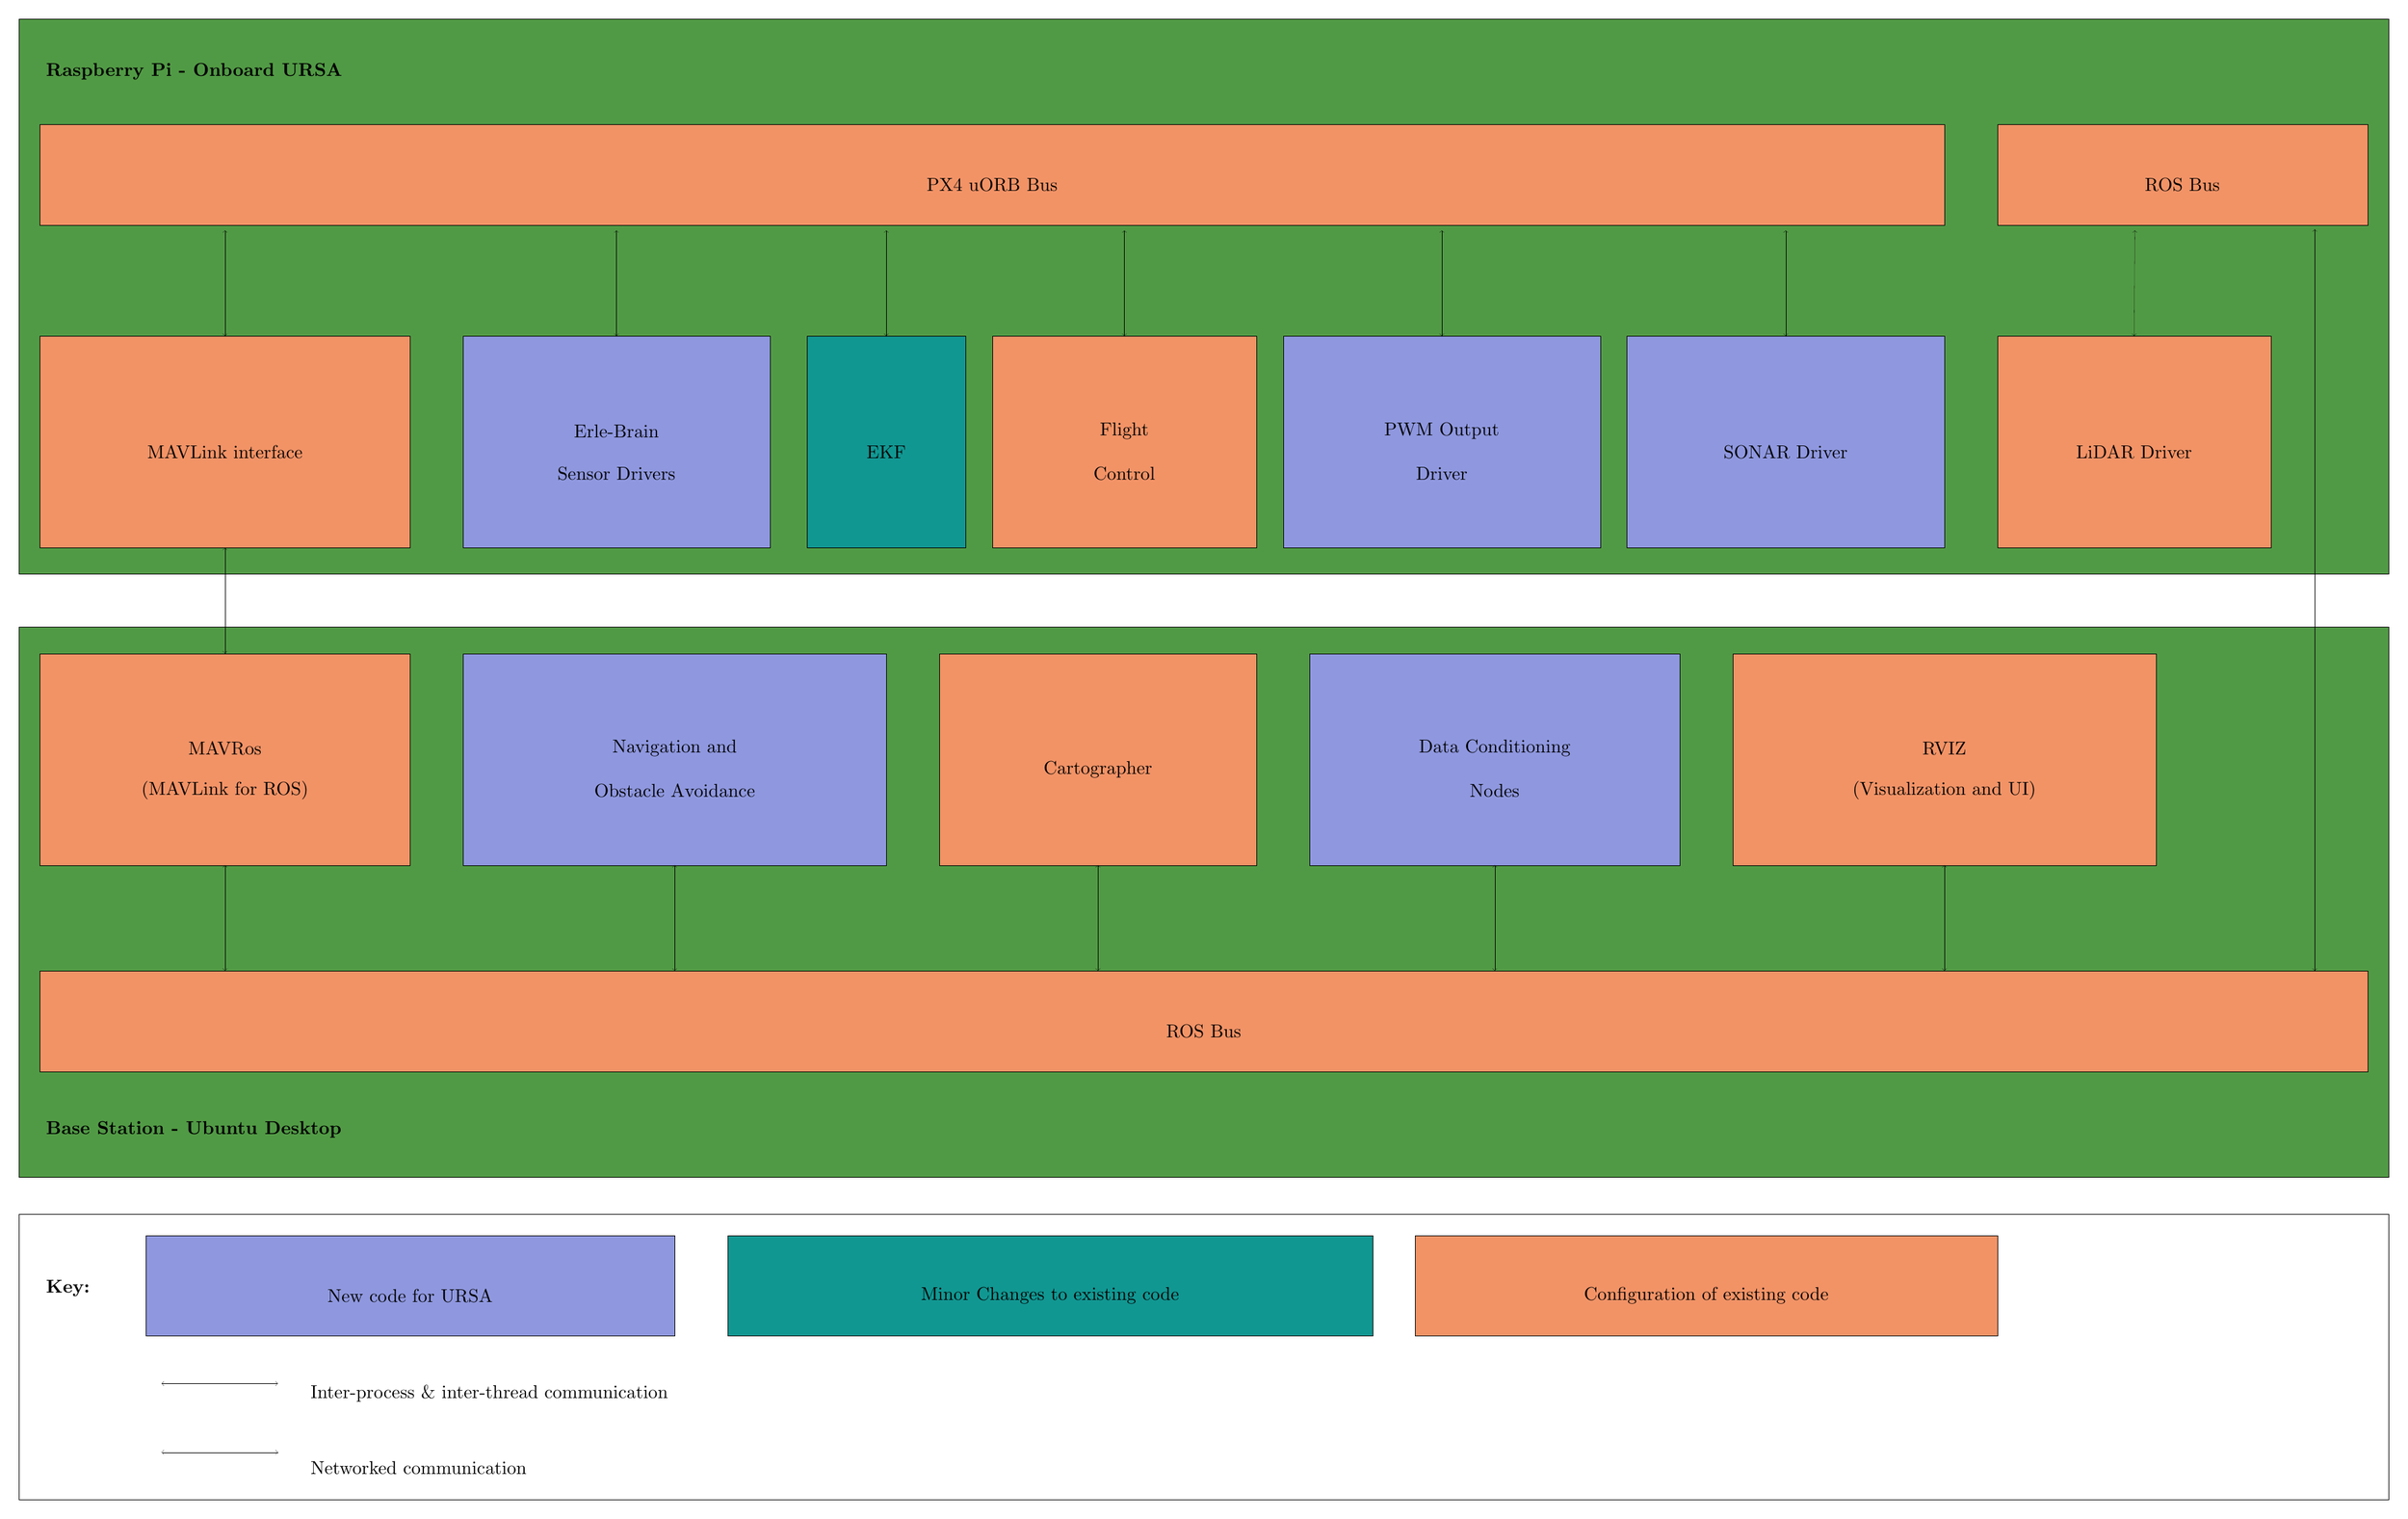
\begin{tikzpicture}
\pgftransformxscale{1.000000}
\pgftransformyscale{-1.000000}
\definecolor{dialinecolor}{rgb}{0.000000, 0.000000, 0.000000}
\pgfsetstrokecolor{dialinecolor}
\definecolor{dialinecolor}{rgb}{1.000000, 1.000000, 1.000000}
\pgfsetfillcolor{dialinecolor}
\pgfsetlinewidth{0.100000\du}
\pgfsetdash{}{0pt}
\pgfsetdash{}{0pt}
\pgfsetmiterjoin
\definecolor{dialinecolor}{rgb}{1.000000, 1.000000, 1.000000}
\pgfsetfillcolor{dialinecolor}
\fill (-1.400000\du,25.600000\du)--(-1.400000\du,31.000000\du)--(43.400000\du,31.000000\du)--(43.400000\du,25.600000\du)--cycle;
\definecolor{dialinecolor}{rgb}{0.000000, 0.000000, 0.000000}
\pgfsetstrokecolor{dialinecolor}
\draw (-1.400000\du,25.600000\du)--(-1.400000\du,31.000000\du)--(43.400000\du,31.000000\du)--(43.400000\du,25.600000\du)--cycle;
\pgfsetlinewidth{0.100000\du}
\pgfsetdash{}{0pt}
\pgfsetdash{}{0pt}
\pgfsetmiterjoin
\definecolor{dialinecolor}{rgb}{0.317647, 0.603922, 0.270588}
\pgfsetfillcolor{dialinecolor}
\fill (-1.400000\du,14.500000\du)--(-1.400000\du,24.900000\du)--(43.400000\du,24.900000\du)--(43.400000\du,14.500000\du)--cycle;
\definecolor{dialinecolor}{rgb}{0.000000, 0.000000, 0.000000}
\pgfsetstrokecolor{dialinecolor}
\draw (-1.400000\du,14.500000\du)--(-1.400000\du,24.900000\du)--(43.400000\du,24.900000\du)--(43.400000\du,14.500000\du)--cycle;
\pgfsetlinewidth{0.100000\du}
\pgfsetdash{}{0pt}
\pgfsetdash{}{0pt}
\pgfsetmiterjoin
\definecolor{dialinecolor}{rgb}{0.317647, 0.603922, 0.270588}
\pgfsetfillcolor{dialinecolor}
\fill (-1.400000\du,3.000000\du)--(-1.400000\du,13.500000\du)--(43.400000\du,13.500000\du)--(43.400000\du,3.000000\du)--cycle;
\definecolor{dialinecolor}{rgb}{0.000000, 0.000000, 0.000000}
\pgfsetstrokecolor{dialinecolor}
\draw (-1.400000\du,3.000000\du)--(-1.400000\du,13.500000\du)--(43.400000\du,13.500000\du)--(43.400000\du,3.000000\du)--cycle;
\definecolor{dialinecolor}{rgb}{0.949020, 0.576471, 0.400000}
\pgfsetfillcolor{dialinecolor}
\fill (-1.000000\du,21.000000\du)--(-1.000000\du,22.900000\du)--(43.000000\du,22.900000\du)--(43.000000\du,21.000000\du)--cycle;
\pgfsetlinewidth{0.100000\du}
\pgfsetdash{}{0pt}
\pgfsetdash{}{0pt}
\pgfsetmiterjoin
\definecolor{dialinecolor}{rgb}{0.000000, 0.000000, 0.000000}
\pgfsetstrokecolor{dialinecolor}
\draw (-1.000000\du,21.000000\du)--(-1.000000\du,22.900000\du)--(43.000000\du,22.900000\du)--(43.000000\du,21.000000\du)--cycle;
% setfont left to latex
\definecolor{dialinecolor}{rgb}{0.000000, 0.000000, 0.000000}
\pgfsetstrokecolor{dialinecolor}
\node at (21.000000\du,22.145000\du){ROS Bus};
\definecolor{dialinecolor}{rgb}{0.949020, 0.576471, 0.400000}
\pgfsetfillcolor{dialinecolor}
\fill (-1.000000\du,15.000000\du)--(-1.000000\du,19.000000\du)--(6.000000\du,19.000000\du)--(6.000000\du,15.000000\du)--cycle;
\pgfsetlinewidth{0.100000\du}
\pgfsetdash{}{0pt}
\pgfsetdash{}{0pt}
\pgfsetmiterjoin
\definecolor{dialinecolor}{rgb}{0.000000, 0.000000, 0.000000}
\pgfsetstrokecolor{dialinecolor}
\draw (-1.000000\du,15.000000\du)--(-1.000000\du,19.000000\du)--(6.000000\du,19.000000\du)--(6.000000\du,15.000000\du)--cycle;
% setfont left to latex
\definecolor{dialinecolor}{rgb}{0.000000, 0.000000, 0.000000}
\pgfsetstrokecolor{dialinecolor}
\node at (2.500000\du,16.795000\du){MAVRos};
% setfont left to latex
\definecolor{dialinecolor}{rgb}{0.000000, 0.000000, 0.000000}
\pgfsetstrokecolor{dialinecolor}
\node at (2.500000\du,17.595000\du){(MAVLink for ROS)};
\definecolor{dialinecolor}{rgb}{0.949020, 0.576471, 0.400000}
\pgfsetfillcolor{dialinecolor}
\fill (16.000000\du,15.000000\du)--(16.000000\du,19.000000\du)--(22.000000\du,19.000000\du)--(22.000000\du,15.000000\du)--cycle;
\pgfsetlinewidth{0.100000\du}
\pgfsetdash{}{0pt}
\pgfsetdash{}{0pt}
\pgfsetmiterjoin
\definecolor{dialinecolor}{rgb}{0.000000, 0.000000, 0.000000}
\pgfsetstrokecolor{dialinecolor}
\draw (16.000000\du,15.000000\du)--(16.000000\du,19.000000\du)--(22.000000\du,19.000000\du)--(22.000000\du,15.000000\du)--cycle;
% setfont left to latex
\definecolor{dialinecolor}{rgb}{0.000000, 0.000000, 0.000000}
\pgfsetstrokecolor{dialinecolor}
\node at (19.000000\du,17.195000\du){Cartographer};
\definecolor{dialinecolor}{rgb}{0.560784, 0.596078, 0.874510}
\pgfsetfillcolor{dialinecolor}
\fill (7.000000\du,15.000000\du)--(7.000000\du,19.000000\du)--(15.000000\du,19.000000\du)--(15.000000\du,15.000000\du)--cycle;
\pgfsetlinewidth{0.100000\du}
\pgfsetdash{}{0pt}
\pgfsetdash{}{0pt}
\pgfsetmiterjoin
\definecolor{dialinecolor}{rgb}{0.000000, 0.000000, 0.000000}
\pgfsetstrokecolor{dialinecolor}
\draw (7.000000\du,15.000000\du)--(7.000000\du,19.000000\du)--(15.000000\du,19.000000\du)--(15.000000\du,15.000000\du)--cycle;
% setfont left to latex
\definecolor{dialinecolor}{rgb}{0.000000, 0.000000, 0.000000}
\pgfsetstrokecolor{dialinecolor}
\node at (11.000000\du,16.795000\du){Navigation and};
% setfont left to latex
\definecolor{dialinecolor}{rgb}{0.000000, 0.000000, 0.000000}
\pgfsetstrokecolor{dialinecolor}
\node at (11.000000\du,17.595000\du){Obstacle Avoidance};
\definecolor{dialinecolor}{rgb}{0.949020, 0.576471, 0.400000}
\pgfsetfillcolor{dialinecolor}
\fill (31.000000\du,15.000000\du)--(31.000000\du,19.000000\du)--(39.000000\du,19.000000\du)--(39.000000\du,15.000000\du)--cycle;
\pgfsetlinewidth{0.100000\du}
\pgfsetdash{}{0pt}
\pgfsetdash{}{0pt}
\pgfsetmiterjoin
\definecolor{dialinecolor}{rgb}{0.000000, 0.000000, 0.000000}
\pgfsetstrokecolor{dialinecolor}
\draw (31.000000\du,15.000000\du)--(31.000000\du,19.000000\du)--(39.000000\du,19.000000\du)--(39.000000\du,15.000000\du)--cycle;
% setfont left to latex
\definecolor{dialinecolor}{rgb}{0.000000, 0.000000, 0.000000}
\pgfsetstrokecolor{dialinecolor}
\node at (35.000000\du,16.795000\du){RVIZ};
% setfont left to latex
\definecolor{dialinecolor}{rgb}{0.000000, 0.000000, 0.000000}
\pgfsetstrokecolor{dialinecolor}
\node at (35.000000\du,17.595000\du){(Visualization and UI)};
\definecolor{dialinecolor}{rgb}{0.949020, 0.576471, 0.400000}
\pgfsetfillcolor{dialinecolor}
\fill (36.000000\du,9.000000\du)--(36.000000\du,13.000000\du)--(41.172500\du,13.000000\du)--(41.172500\du,9.000000\du)--cycle;
\pgfsetlinewidth{0.100000\du}
\pgfsetdash{}{0pt}
\pgfsetdash{}{0pt}
\pgfsetmiterjoin
\definecolor{dialinecolor}{rgb}{0.000000, 0.000000, 0.000000}
\pgfsetstrokecolor{dialinecolor}
\draw (36.000000\du,9.000000\du)--(36.000000\du,13.000000\du)--(41.172500\du,13.000000\du)--(41.172500\du,9.000000\du)--cycle;
% setfont left to latex
\definecolor{dialinecolor}{rgb}{0.000000, 0.000000, 0.000000}
\pgfsetstrokecolor{dialinecolor}
\node at (38.586250\du,11.195000\du){LiDAR Driver};
\definecolor{dialinecolor}{rgb}{0.949020, 0.576471, 0.400000}
\pgfsetfillcolor{dialinecolor}
\fill (-1.000000\du,9.000000\du)--(-1.000000\du,13.000000\du)--(6.000000\du,13.000000\du)--(6.000000\du,9.000000\du)--cycle;
\pgfsetlinewidth{0.100000\du}
\pgfsetdash{}{0pt}
\pgfsetdash{}{0pt}
\pgfsetmiterjoin
\definecolor{dialinecolor}{rgb}{0.000000, 0.000000, 0.000000}
\pgfsetstrokecolor{dialinecolor}
\draw (-1.000000\du,9.000000\du)--(-1.000000\du,13.000000\du)--(6.000000\du,13.000000\du)--(6.000000\du,9.000000\du)--cycle;
% setfont left to latex
\definecolor{dialinecolor}{rgb}{0.000000, 0.000000, 0.000000}
\pgfsetstrokecolor{dialinecolor}
\node at (2.500000\du,11.195000\du){MAVLink interface};
\definecolor{dialinecolor}{rgb}{0.560784, 0.596078, 0.874510}
\pgfsetfillcolor{dialinecolor}
\fill (7.000000\du,9.000000\du)--(7.000000\du,13.000000\du)--(12.800000\du,13.000000\du)--(12.800000\du,9.000000\du)--cycle;
\pgfsetlinewidth{0.100000\du}
\pgfsetdash{}{0pt}
\pgfsetdash{}{0pt}
\pgfsetmiterjoin
\definecolor{dialinecolor}{rgb}{0.000000, 0.000000, 0.000000}
\pgfsetstrokecolor{dialinecolor}
\draw (7.000000\du,9.000000\du)--(7.000000\du,13.000000\du)--(12.800000\du,13.000000\du)--(12.800000\du,9.000000\du)--cycle;
% setfont left to latex
\definecolor{dialinecolor}{rgb}{0.000000, 0.000000, 0.000000}
\pgfsetstrokecolor{dialinecolor}
\node at (9.900000\du,10.795000\du){Erle-Brain};
% setfont left to latex
\definecolor{dialinecolor}{rgb}{0.000000, 0.000000, 0.000000}
\pgfsetstrokecolor{dialinecolor}
\node at (9.900000\du,11.595000\du){Sensor Drivers};
\definecolor{dialinecolor}{rgb}{0.560784, 0.596078, 0.874510}
\pgfsetfillcolor{dialinecolor}
\fill (29.000000\du,9.000000\du)--(29.000000\du,13.000000\du)--(35.000000\du,13.000000\du)--(35.000000\du,9.000000\du)--cycle;
\pgfsetlinewidth{0.100000\du}
\pgfsetdash{}{0pt}
\pgfsetdash{}{0pt}
\pgfsetmiterjoin
\definecolor{dialinecolor}{rgb}{0.000000, 0.000000, 0.000000}
\pgfsetstrokecolor{dialinecolor}
\draw (29.000000\du,9.000000\du)--(29.000000\du,13.000000\du)--(35.000000\du,13.000000\du)--(35.000000\du,9.000000\du)--cycle;
% setfont left to latex
\definecolor{dialinecolor}{rgb}{0.000000, 0.000000, 0.000000}
\pgfsetstrokecolor{dialinecolor}
\node at (32.000000\du,11.195000\du){SONAR Driver};
\definecolor{dialinecolor}{rgb}{0.949020, 0.576471, 0.400000}
\pgfsetfillcolor{dialinecolor}
\fill (-1.000000\du,5.000000\du)--(-1.000000\du,6.900000\du)--(35.000000\du,6.900000\du)--(35.000000\du,5.000000\du)--cycle;
\pgfsetlinewidth{0.100000\du}
\pgfsetdash{}{0pt}
\pgfsetdash{}{0pt}
\pgfsetmiterjoin
\definecolor{dialinecolor}{rgb}{0.000000, 0.000000, 0.000000}
\pgfsetstrokecolor{dialinecolor}
\draw (-1.000000\du,5.000000\du)--(-1.000000\du,6.900000\du)--(35.000000\du,6.900000\du)--(35.000000\du,5.000000\du)--cycle;
% setfont left to latex
\definecolor{dialinecolor}{rgb}{0.000000, 0.000000, 0.000000}
\pgfsetstrokecolor{dialinecolor}
\node at (17.000000\du,6.145000\du){PX4 uORB Bus};
\definecolor{dialinecolor}{rgb}{0.066667, 0.592157, 0.572549}
\pgfsetfillcolor{dialinecolor}
\fill (13.500000\du,9.000000\du)--(13.500000\du,13.000000\du)--(16.500000\du,13.000000\du)--(16.500000\du,9.000000\du)--cycle;
\pgfsetlinewidth{0.100000\du}
\pgfsetdash{}{0pt}
\pgfsetdash{}{0pt}
\pgfsetmiterjoin
\definecolor{dialinecolor}{rgb}{0.000000, 0.000000, 0.000000}
\pgfsetstrokecolor{dialinecolor}
\draw (13.500000\du,9.000000\du)--(13.500000\du,13.000000\du)--(16.500000\du,13.000000\du)--(16.500000\du,9.000000\du)--cycle;
% setfont left to latex
\definecolor{dialinecolor}{rgb}{0.000000, 0.000000, 0.000000}
\pgfsetstrokecolor{dialinecolor}
\node at (15.000000\du,11.195000\du){EKF};
\definecolor{dialinecolor}{rgb}{0.560784, 0.596078, 0.874510}
\pgfsetfillcolor{dialinecolor}
\fill (22.500000\du,9.000000\du)--(22.500000\du,13.000000\du)--(28.500000\du,13.000000\du)--(28.500000\du,9.000000\du)--cycle;
\pgfsetlinewidth{0.100000\du}
\pgfsetdash{}{0pt}
\pgfsetdash{}{0pt}
\pgfsetmiterjoin
\definecolor{dialinecolor}{rgb}{0.000000, 0.000000, 0.000000}
\pgfsetstrokecolor{dialinecolor}
\draw (22.500000\du,9.000000\du)--(22.500000\du,13.000000\du)--(28.500000\du,13.000000\du)--(28.500000\du,9.000000\du)--cycle;
% setfont left to latex
\definecolor{dialinecolor}{rgb}{0.000000, 0.000000, 0.000000}
\pgfsetstrokecolor{dialinecolor}
\node at (25.500000\du,10.795000\du){PWM Output};
% setfont left to latex
\definecolor{dialinecolor}{rgb}{0.000000, 0.000000, 0.000000}
\pgfsetstrokecolor{dialinecolor}
\node at (25.500000\du,11.595000\du){Driver};
\definecolor{dialinecolor}{rgb}{0.560784, 0.596078, 0.874510}
\pgfsetfillcolor{dialinecolor}
\fill (23.000000\du,15.000000\du)--(23.000000\du,19.000000\du)--(30.000000\du,19.000000\du)--(30.000000\du,15.000000\du)--cycle;
\pgfsetlinewidth{0.100000\du}
\pgfsetdash{}{0pt}
\pgfsetdash{}{0pt}
\pgfsetmiterjoin
\definecolor{dialinecolor}{rgb}{0.000000, 0.000000, 0.000000}
\pgfsetstrokecolor{dialinecolor}
\draw (23.000000\du,15.000000\du)--(23.000000\du,19.000000\du)--(30.000000\du,19.000000\du)--(30.000000\du,15.000000\du)--cycle;
% setfont left to latex
\definecolor{dialinecolor}{rgb}{0.000000, 0.000000, 0.000000}
\pgfsetstrokecolor{dialinecolor}
\node at (26.500000\du,16.795000\du){Data Conditioning};
% setfont left to latex
\definecolor{dialinecolor}{rgb}{0.000000, 0.000000, 0.000000}
\pgfsetstrokecolor{dialinecolor}
\node at (26.500000\du,17.595000\du){Nodes};
\definecolor{dialinecolor}{rgb}{0.949020, 0.576471, 0.400000}
\pgfsetfillcolor{dialinecolor}
\fill (17.000000\du,9.000000\du)--(17.000000\du,13.000000\du)--(22.000000\du,13.000000\du)--(22.000000\du,9.000000\du)--cycle;
\pgfsetlinewidth{0.100000\du}
\pgfsetdash{}{0pt}
\pgfsetdash{}{0pt}
\pgfsetmiterjoin
\definecolor{dialinecolor}{rgb}{0.000000, 0.000000, 0.000000}
\pgfsetstrokecolor{dialinecolor}
\draw (17.000000\du,9.000000\du)--(17.000000\du,13.000000\du)--(22.000000\du,13.000000\du)--(22.000000\du,9.000000\du)--cycle;
% setfont left to latex
\definecolor{dialinecolor}{rgb}{0.000000, 0.000000, 0.000000}
\pgfsetstrokecolor{dialinecolor}
\node at (19.500000\du,10.795000\du){Flight};
% setfont left to latex
\definecolor{dialinecolor}{rgb}{0.000000, 0.000000, 0.000000}
\pgfsetstrokecolor{dialinecolor}
\node at (19.500000\du,11.595000\du){Control};
\pgfsetlinewidth{0.100000\du}
\pgfsetdash{}{0pt}
\pgfsetdash{}{0pt}
\pgfsetbuttcap
{
\definecolor{dialinecolor}{rgb}{0.000000, 0.000000, 0.000000}
\pgfsetfillcolor{dialinecolor}
% was here!!!
\pgfsetarrowsstart{to}
\pgfsetarrowsend{to}
\definecolor{dialinecolor}{rgb}{0.000000, 0.000000, 0.000000}
\pgfsetstrokecolor{dialinecolor}
\draw (2.500000\du,9.000000\du)--(2.500000\du,7.000000\du);
}
\pgfsetlinewidth{0.100000\du}
\pgfsetdash{}{0pt}
\pgfsetdash{}{0pt}
\pgfsetbuttcap
{
\definecolor{dialinecolor}{rgb}{0.000000, 0.000000, 0.000000}
\pgfsetfillcolor{dialinecolor}
% was here!!!
\pgfsetarrowsstart{to}
\pgfsetarrowsend{to}
\definecolor{dialinecolor}{rgb}{0.000000, 0.000000, 0.000000}
\pgfsetstrokecolor{dialinecolor}
\draw (9.900000\du,9.000000\du)--(9.900000\du,7.000000\du);
}
\pgfsetlinewidth{0.100000\du}
\pgfsetdash{}{0pt}
\pgfsetdash{}{0pt}
\pgfsetbuttcap
{
\definecolor{dialinecolor}{rgb}{0.000000, 0.000000, 0.000000}
\pgfsetfillcolor{dialinecolor}
% was here!!!
\pgfsetarrowsstart{to}
\pgfsetarrowsend{to}
\definecolor{dialinecolor}{rgb}{0.000000, 0.000000, 0.000000}
\pgfsetstrokecolor{dialinecolor}
\draw (15.000000\du,9.000000\du)--(15.000000\du,7.000000\du);
}
\pgfsetlinewidth{0.100000\du}
\pgfsetdash{}{0pt}
\pgfsetdash{}{0pt}
\pgfsetbuttcap
{
\definecolor{dialinecolor}{rgb}{0.000000, 0.000000, 0.000000}
\pgfsetfillcolor{dialinecolor}
% was here!!!
\pgfsetarrowsstart{to}
\pgfsetarrowsend{to}
\definecolor{dialinecolor}{rgb}{0.000000, 0.000000, 0.000000}
\pgfsetstrokecolor{dialinecolor}
\draw (19.500000\du,9.000000\du)--(19.500000\du,7.000000\du);
}
\pgfsetlinewidth{0.100000\du}
\pgfsetdash{}{0pt}
\pgfsetdash{}{0pt}
\pgfsetbuttcap
{
\definecolor{dialinecolor}{rgb}{0.000000, 0.000000, 0.000000}
\pgfsetfillcolor{dialinecolor}
% was here!!!
\pgfsetarrowsstart{to}
\pgfsetarrowsend{to}
\definecolor{dialinecolor}{rgb}{0.000000, 0.000000, 0.000000}
\pgfsetstrokecolor{dialinecolor}
\draw (25.500000\du,9.000000\du)--(25.500000\du,7.000000\du);
}
\pgfsetlinewidth{0.100000\du}
\pgfsetdash{}{0pt}
\pgfsetdash{}{0pt}
\pgfsetbuttcap
{
\definecolor{dialinecolor}{rgb}{0.000000, 0.000000, 0.000000}
\pgfsetfillcolor{dialinecolor}
% was here!!!
\pgfsetarrowsstart{to}
\pgfsetarrowsend{to}
\definecolor{dialinecolor}{rgb}{0.000000, 0.000000, 0.000000}
\pgfsetstrokecolor{dialinecolor}
\draw (32.000000\du,9.000000\du)--(32.000000\du,7.000000\du);
}
\pgfsetlinewidth{0.100000\du}
\pgfsetdash{{\pgflinewidth}{0.200000\du}}{0cm}
\pgfsetdash{{\pgflinewidth}{0.200000\du}}{0cm}
\pgfsetbuttcap
{
\definecolor{dialinecolor}{rgb}{0.000000, 0.000000, 0.000000}
\pgfsetfillcolor{dialinecolor}
% was here!!!
\pgfsetarrowsstart{to}
\pgfsetarrowsend{to}
\definecolor{dialinecolor}{rgb}{0.000000, 0.000000, 0.000000}
\pgfsetstrokecolor{dialinecolor}
\draw (2.500000\du,15.000000\du)--(2.500000\du,13.000000\du);
}
\pgfsetlinewidth{0.100000\du}
\pgfsetdash{{\pgflinewidth}{0.200000\du}}{0cm}
\pgfsetdash{{\pgflinewidth}{0.200000\du}}{0cm}
\pgfsetbuttcap
{
\definecolor{dialinecolor}{rgb}{0.000000, 0.000000, 0.000000}
\pgfsetfillcolor{dialinecolor}
% was here!!!
\pgfsetarrowsstart{to}
\pgfsetarrowsend{to}
\definecolor{dialinecolor}{rgb}{0.000000, 0.000000, 0.000000}
\pgfsetstrokecolor{dialinecolor}
\draw (42.000000\du,21.000000\du)--(42.000000\du,6.980000\du);
}
\definecolor{dialinecolor}{rgb}{0.949020, 0.576471, 0.400000}
\pgfsetfillcolor{dialinecolor}
\fill (36.000000\du,5.000000\du)--(36.000000\du,6.900000\du)--(43.000000\du,6.900000\du)--(43.000000\du,5.000000\du)--cycle;
\pgfsetlinewidth{0.100000\du}
\pgfsetdash{}{0pt}
\pgfsetdash{}{0pt}
\pgfsetmiterjoin
\definecolor{dialinecolor}{rgb}{0.000000, 0.000000, 0.000000}
\pgfsetstrokecolor{dialinecolor}
\draw (36.000000\du,5.000000\du)--(36.000000\du,6.900000\du)--(43.000000\du,6.900000\du)--(43.000000\du,5.000000\du)--cycle;
% setfont left to latex
\definecolor{dialinecolor}{rgb}{0.000000, 0.000000, 0.000000}
\pgfsetstrokecolor{dialinecolor}
\node at (39.500000\du,6.145000\du){ROS Bus};
\pgfsetlinewidth{0.100000\du}
\pgfsetdash{}{0pt}
\pgfsetdash{}{0pt}
\pgfsetbuttcap
{
\definecolor{dialinecolor}{rgb}{0.000000, 0.000000, 0.000000}
\pgfsetfillcolor{dialinecolor}
% was here!!!
\pgfsetarrowsstart{to}
\pgfsetarrowsend{to}
\definecolor{dialinecolor}{rgb}{0.000000, 0.000000, 0.000000}
\pgfsetstrokecolor{dialinecolor}
\draw (38.586250\du,9.000000\du)--(38.600000\du,7.000000\du);
}
\pgfsetlinewidth{0.100000\du}
\pgfsetdash{}{0pt}
\pgfsetdash{}{0pt}
\pgfsetbuttcap
{
\definecolor{dialinecolor}{rgb}{0.000000, 0.000000, 0.000000}
\pgfsetfillcolor{dialinecolor}
% was here!!!
\pgfsetarrowsstart{to}
\pgfsetarrowsend{to}
\definecolor{dialinecolor}{rgb}{0.000000, 0.000000, 0.000000}
\pgfsetstrokecolor{dialinecolor}
\draw (2.500000\du,21.000000\du)--(2.500000\du,19.000000\du);
}
\pgfsetlinewidth{0.100000\du}
\pgfsetdash{}{0pt}
\pgfsetdash{}{0pt}
\pgfsetbuttcap
{
\definecolor{dialinecolor}{rgb}{0.000000, 0.000000, 0.000000}
\pgfsetfillcolor{dialinecolor}
% was here!!!
\pgfsetarrowsstart{to}
\pgfsetarrowsend{to}
\definecolor{dialinecolor}{rgb}{0.000000, 0.000000, 0.000000}
\pgfsetstrokecolor{dialinecolor}
\draw (11.000000\du,21.000000\du)--(11.000000\du,19.000000\du);
}
\pgfsetlinewidth{0.100000\du}
\pgfsetdash{}{0pt}
\pgfsetdash{}{0pt}
\pgfsetbuttcap
{
\definecolor{dialinecolor}{rgb}{0.000000, 0.000000, 0.000000}
\pgfsetfillcolor{dialinecolor}
% was here!!!
\pgfsetarrowsstart{to}
\pgfsetarrowsend{to}
\definecolor{dialinecolor}{rgb}{0.000000, 0.000000, 0.000000}
\pgfsetstrokecolor{dialinecolor}
\draw (19.000000\du,21.000000\du)--(19.000000\du,19.000000\du);
}
\pgfsetlinewidth{0.100000\du}
\pgfsetdash{}{0pt}
\pgfsetdash{}{0pt}
\pgfsetbuttcap
{
\definecolor{dialinecolor}{rgb}{0.000000, 0.000000, 0.000000}
\pgfsetfillcolor{dialinecolor}
% was here!!!
\pgfsetarrowsstart{to}
\pgfsetarrowsend{to}
\definecolor{dialinecolor}{rgb}{0.000000, 0.000000, 0.000000}
\pgfsetstrokecolor{dialinecolor}
\draw (26.500000\du,21.000000\du)--(26.500000\du,19.000000\du);
}
\pgfsetlinewidth{0.100000\du}
\pgfsetdash{}{0pt}
\pgfsetdash{}{0pt}
\pgfsetbuttcap
{
\definecolor{dialinecolor}{rgb}{0.000000, 0.000000, 0.000000}
\pgfsetfillcolor{dialinecolor}
% was here!!!
\pgfsetarrowsstart{to}
\pgfsetarrowsend{to}
\definecolor{dialinecolor}{rgb}{0.000000, 0.000000, 0.000000}
\pgfsetstrokecolor{dialinecolor}
\draw (35.000000\du,21.000000\du)--(35.000000\du,19.000000\du);
}
% setfont left to latex
\definecolor{dialinecolor}{rgb}{0.000000, 0.000000, 0.000000}
\pgfsetstrokecolor{dialinecolor}
\node[anchor=west] at (21.000000\du,8.250000\du){};
% setfont left to latex
\definecolor{dialinecolor}{rgb}{0.000000, 0.000000, 0.000000}
\pgfsetstrokecolor{dialinecolor}
\node[anchor=west] at (-1.000000\du,4.000000\du){\bf Raspberry Pi - Onboard URSA};
% setfont left to latex
\definecolor{dialinecolor}{rgb}{0.000000, 0.000000, 0.000000}
\pgfsetstrokecolor{dialinecolor}
\node[anchor=west] at (-1.000000\du,24.000000\du){\bf Base Station - Ubuntu Desktop};
% setfont left to latex
\definecolor{dialinecolor}{rgb}{0.000000, 0.000000, 0.000000}
\pgfsetstrokecolor{dialinecolor}
\node[anchor=west] at (-1.000000\du,27.000000\du){\bf Key:};
\definecolor{dialinecolor}{rgb}{0.560784, 0.596078, 0.874510}
\pgfsetfillcolor{dialinecolor}
\fill (1.000000\du,26.000000\du)--(1.000000\du,27.900000\du)--(11.000000\du,27.900000\du)--(11.000000\du,26.000000\du)--cycle;
\pgfsetlinewidth{0.100000\du}
\pgfsetdash{}{0pt}
\pgfsetdash{}{0pt}
\pgfsetmiterjoin
\definecolor{dialinecolor}{rgb}{0.000000, 0.000000, 0.000000}
\pgfsetstrokecolor{dialinecolor}
\draw (1.000000\du,26.000000\du)--(1.000000\du,27.900000\du)--(11.000000\du,27.900000\du)--(11.000000\du,26.000000\du)--cycle;
% setfont left to latex
\definecolor{dialinecolor}{rgb}{0.000000, 0.000000, 0.000000}
\pgfsetstrokecolor{dialinecolor}
\node at (6.000000\du,27.145000\du){New code for URSA};
\definecolor{dialinecolor}{rgb}{0.066667, 0.592157, 0.572549}
\pgfsetfillcolor{dialinecolor}
\fill (12.000000\du,26.000000\du)--(12.000000\du,27.900000\du)--(24.190000\du,27.900000\du)--(24.190000\du,26.000000\du)--cycle;
\pgfsetlinewidth{0.100000\du}
\pgfsetdash{}{0pt}
\pgfsetdash{}{0pt}
\pgfsetmiterjoin
\definecolor{dialinecolor}{rgb}{0.000000, 0.000000, 0.000000}
\pgfsetstrokecolor{dialinecolor}
\draw (12.000000\du,26.000000\du)--(12.000000\du,27.900000\du)--(24.190000\du,27.900000\du)--(24.190000\du,26.000000\du)--cycle;
% setfont left to latex
\definecolor{dialinecolor}{rgb}{0.000000, 0.000000, 0.000000}
\pgfsetstrokecolor{dialinecolor}
\node at (18.095000\du,27.145000\du){Minor Changes to existing code};
\definecolor{dialinecolor}{rgb}{0.949020, 0.576471, 0.400000}
\pgfsetfillcolor{dialinecolor}
\fill (25.000000\du,26.000000\du)--(25.000000\du,27.900000\du)--(36.000000\du,27.900000\du)--(36.000000\du,26.000000\du)--cycle;
\pgfsetlinewidth{0.100000\du}
\pgfsetdash{}{0pt}
\pgfsetdash{}{0pt}
\pgfsetmiterjoin
\definecolor{dialinecolor}{rgb}{0.000000, 0.000000, 0.000000}
\pgfsetstrokecolor{dialinecolor}
\draw (25.000000\du,26.000000\du)--(25.000000\du,27.900000\du)--(36.000000\du,27.900000\du)--(36.000000\du,26.000000\du)--cycle;
% setfont left to latex
\definecolor{dialinecolor}{rgb}{0.000000, 0.000000, 0.000000}
\pgfsetstrokecolor{dialinecolor}
\node at (30.500000\du,27.145000\du){Configuration of existing code};
\pgfsetlinewidth{0.100000\du}
\pgfsetdash{}{0pt}
\pgfsetdash{}{0pt}
\pgfsetbuttcap
{
\definecolor{dialinecolor}{rgb}{0.000000, 0.000000, 0.000000}
\pgfsetfillcolor{dialinecolor}
% was here!!!
\pgfsetarrowsstart{to}
\pgfsetarrowsend{to}
\definecolor{dialinecolor}{rgb}{0.000000, 0.000000, 0.000000}
\pgfsetstrokecolor{dialinecolor}
\draw (3.500000\du,28.800000\du)--(1.300000\du,28.800000\du);
}
\pgfsetlinewidth{0.100000\du}
\pgfsetdash{{\pgflinewidth}{0.200000\du}}{0cm}
\pgfsetdash{{\pgflinewidth}{0.200000\du}}{0cm}
\pgfsetbuttcap
{
\definecolor{dialinecolor}{rgb}{0.000000, 0.000000, 0.000000}
\pgfsetfillcolor{dialinecolor}
% was here!!!
\pgfsetarrowsstart{to}
\pgfsetarrowsend{to}
\definecolor{dialinecolor}{rgb}{0.000000, 0.000000, 0.000000}
\pgfsetstrokecolor{dialinecolor}
\draw (3.500000\du,30.100000\du)--(1.300000\du,30.100000\du);
}
% setfont left to latex
\definecolor{dialinecolor}{rgb}{0.000000, 0.000000, 0.000000}
\pgfsetstrokecolor{dialinecolor}
\node[anchor=west] at (4.000000\du,29.000000\du){Inter-process \& inter-thread communication};
% setfont left to latex
\definecolor{dialinecolor}{rgb}{0.000000, 0.000000, 0.000000}
\pgfsetstrokecolor{dialinecolor}
\node[anchor=west] at (4.000000\du,30.400000\du){Networked communication};
\end{tikzpicture}

	\caption{Overall URSA system architecture\label{fig:overArch}}
\end{figure}
\vfill
\end{landscape}
\pagebreak


\end{document}
